\documentclass[10pt,a4paper]{scrartcl}

\usepackage[ngerman]{babel}

\newlength{\mylength}
\setlength{\mylength}{.6	 cm}
\usepackage[landscape, top=\mylength, bottom=\mylength, left=\mylength, right=\mylength,includefoot,foot=.6cm]{geometry} %pagelayout

\usepackage[utf8]{inputenc} %language
\usepackage{graphicx} %include pictures
% tables & layout
\usepackage{tabulary} %tables with linebreaks
\usepackage{tabularx}
\usepackage{multicol} %multiple columns
\usepackage{multirow} %connect cells of tabular vertically
\usepackage{bigdelim}
\usepackage{array}   % for \newcolumntype macro
\usepackage{enumerate}
\usepackage{enumitem} %change spaces between listed items [itemsep = x pt]
% math
\usepackage{amsmath} %advanced mathematics
\usepackage{amssymb} %math symbols
\usepackage[load=prefixed,load=abbr]{siunitx} %use units
\usepackage{mathrsfs} % used for mathscript
\usepackage{mathtools} %use of rcases*
\usepackage{esint} %special integrals

%style
\usepackage[x11names]{xcolor} %colors for titles
\usepackage{soulutf8}
\usepackage{rotating}
% Algorithms
\usepackage{algorithm}
\usepackage{algpseudocode}
\usepackage{listingsutf8}%use of other languages

\usepackage{hyperref}

% Set the color of your style
% Avaiable are: Apricot, Aquamarine, Bittersweet, Black, Blue, blue, BlueGreen, BlueViolet, BrickRed, Brown, BurntOrange, CadetBlue, CarnationPink, Cerulean, CornflowerBlue, Cyan, Dandelion, DarkOrchid, Emerald, ForestGreen, Fuchsia, Goldenrod, Gray, Green, GreenYellow, JungleGreen, Lavender, ... (more at: http://en.wikibooks.org/wiki/LaTeX/Colors)
\def\StyleColor{Snow4}

% section color box
\setkomafont{section}{\mysection}

\newcommand{\mysection}[1]{	
	\Large\normalfont\scshape
    \setlength{\fboxsep}{0cm}%already boxed
    \vspace{0ex}
    \colorbox{\StyleColor!60}{%
        \begin{minipage}{\linewidth}%
            \vspace*{4pt}%Space before
            #1
            \vspace*{4pt}%Space after
        \end{minipage}%
     }
     \vspace{-1ex}
}

%subsection color box
\setkomafont{subsection}{\mysubsection}

\newcommand{\mysubsection}[1]{%
    \normalsize\normalfont\scshape%
    \vspace{-2ex}
    \setlength{\fboxsep}{0cm}%already boxed
    \colorbox{\StyleColor!40}{%
        \begin{minipage}{\linewidth}%
            \vspace*{4pt}%Space before
             #1
            \vspace*{4pt}%Space after
        \end{minipage}%
    }
    \vspace{-2ex}
}
  
\setkomafont{subsubsection}{\mysubsection}
\newcommand{\mysubsubsection}[1]{%
    \small\normalfont\scshape%
    \vspace{-2ex}
    \setlength{\fboxsep}{0cm}%already boxed
    \colorbox{\StyleColor!5}{%
        \begin{minipage}{\linewidth}%
            \vspace*{4pt}%Space before
             #1
            \vspace*{4pt}%Space after
        \end{minipage}%
    }
    \vspace{-2ex}
}
\newcommand{\finn}{\vspace{1.5ex}}

\newcommand{\fix}{\vspace{-23pt}} %reduce wasted space

\newcommand{\Eofr}{\vec{E}\left(\vec{r}\right)} 	%Elektrisches Feld

\newcommand{\Bofr}{\vec{B}\left(\vec{r}\right)}	%Magnetisches Feld

\newcommand{\Hofr}{\vec{H}\left(\vec{r}\right)}	%Magnetische Erregung

\newcommand{\Fofr}{\vec{F}\left(\vec{r}\right)}	%Kraftfeld

\newcommand{\Vprod}[2]{\vec{#1}\times\vec{#2}} 	%Vektorprodukt

\newcommand{\dahe}{$\rightarrow$ }	%easy arrow outside mathmode

\newcommand{\compaq}{\setlength{\itemsep}{-1mm}\setlength{\parskip}{0cm}}%compact itemizes

\newcommand{\ncompaq}{\setlength{\itemsep}{1mm}\setlength{\parskip}{0cm}}%compact itemizes

\newcommand{\mypic}[1]{\includegraphics[width=\linewidth]{#1}} %easy including of pictures within the column

\newcommand{\hfull}{\hfill$|$\hfill} %easy seperation of two equations
%end commands

\newcommand{\longeq}{\hfill$=$\hfill}%easy seperation of an equation

\newcommand{\intinf}[1]{\int_{-\infty}^\infty{#1}}

\newcommand{\expval}[1]{\langle #1\rangle}

\newcommand{\important}[1]{\begin{center}\fbox{#1}\end{center}}

\newcommand{\importname}[2]{\begin{center}\fbox{#2}  #1\end{center}}

\newcommand{\mimportant}[1]{\begin{center}\begin{tabular}{|c|}\hline #1 \\ \hline\end{tabular}\end{center}}

\newcommand{\importable}[1]{\begin{center}\begin{tabular}{|ll|}\hline #1 \\ \hline\end{tabular}\end{center}}

\newcommand{\importabflex}[2]{\begin{center}\begin{tabular}{|#1|}\hline #2\\ \hline\end{tabular}\end{center}}

\newcommand{\mportant}[1]{\begin{center}#1\end{center}}

\newcommand{\mportname}[2]{\begin{center}#2$\quad$#1\end{center}}

\newcommand{\mmportant}[1]{\begin{center}\begin{tabular}{c} #1 \end{tabular}\end{center}}

\newcommand{\mportable}[1]{\begin{center}\begin{tabular}{ll}#1\end{tabular}\end{center}}

\newcommand{\mportabflex}[2]{\begin{center}\begin{tabular}{#1}#2\end{tabular}\end{center}}

\newcommand{\note}[1]{\footnotesize #1 \normalsize}

\newcommand{\notelist}[1]{\footnotesize \begin{itemize}\compaq #1\end{itemize}\normalsize}

\newcommand{\lstfill}{\vspace{4ex}}

\newcommand{\inp}[2]{\langle #1 | #2 \rangle} % fast inner product

\newcommand{\bra}[1]{\langle #1 |}

\newcommand{\ket}[1]{| #1 \rangle}

\newenvironment{brsm}{% % short for 'bracketed small matrix'
  \bigl( \begin{smallmatrix} }{\end{smallmatrix} \bigr)}

\newcommand{\vectwo}[2]{\begin{brsm}#1 \\ #2\end{brsm}}

\newcommand{\element}[2]{\in\mathbb{R}^{#1 \times #2}}

\newcommand{\dive}{\vec{\nabla}\cdot}

\newcommand{\rota}{\vec{\nabla}\times}

\newcommand{\ddt}{\frac{d}{dt}}

\newcommand{\onha}{\frac{1}{2}}

\DeclareRobustCommand{\hlcyan}[1]{{\sethlcolor{Aquamarine1}\hl{#1}}}

\DeclareRobustCommand{\hlyellow}[1]{{\sethlcolor{Yellow1}\hl{#1}}}

\DeclareRobustCommand{\hlpink}[1]{{\sethlcolor{Orchid1}\hl{#1}}}

\DeclareRobustCommand{\hlgreen}[1]{{\sethlcolor{PaleGreen1}\hl{#1}}}

\DeclarePairedDelimiter\ceil{\lceil}{\rceil}

\DeclarePairedDelimiter\floor{\lfloor}{\rfloor}

\newcommand{\prob}[1]{\mathbb{P}(#1)}

\newcommand{\expe}[1]{\mathbb{E}[#1]}

\newcommand{\var}[1]{\text{Var}(#1)}

\newcommand{\cov}[1]{\text{Cov}(#1)}

\newcommand{\corr}[1]{\text{Corr}(#1)}

\newcommand{\sign}[1]{\text{sign}(#1)}

\newcommand{\vtabfill}{\vspace{-0.7ex}$\ $}

\newcommand{\lap}[1]{\mathcal{L}(#1)}

\newcommand{\sinc}{\text{sinc}}

\newcommand{\sbs}[4]{\begin{minipage}[t!]{#1\linewidth}#3\end{minipage}\begin{minipage}[t!]{#2\linewidth}#4\end{minipage}}

\newcommand{\sbss}[2]{\sbs{0.45}{0.45}{#1}{#2}}


\parindent 0pt

\title{System Modeling}
\author{GianAndrea Müller}

\begin{document}

\begin{multicols*}{4}
\maketitle
\tableofcontents
\end{multicols*}

\newpage

Intentionally left blank by Christof Perren.

\newpage

\begin{multicols*}{3}

\section{Basics}

\mypic{System}

\begin{align*}
\dot{x}(t)&=f(x(t),u(t),t),&x(t)\in\mathbb{R}^n,\ u(t)\in\mathbb{R}^m\\
y(t)&=g(x(t),u(t),t),&y(t)\in\mathbb{R}^p
\end{align*}


Transfer function:

\small
$Y(s)=\left[D+C(s\cdot I-A)^{-1}B\right]U(s),\quad y(t)\in\mathbb{C}^p,\ u(t)\in\mathbb{C}^m$\normalsize

\subsection{Model types}

\begin{itemize}
\item \textbf{black box model:} derived from experiments only
\item \textbf{grey-box model:} model-based, experiments need for parameter identification, model variation
\item \textbf{white-box model:} no experiments at all
\end{itemize}

Describing a system by a model based on physical principles allows to \textbf{extrapolate the system behaviour} and is useful if \text{the real system is not available}.

\subsection{Parametric model}

Using a physical model describing the system.

\mypic{Model}

\importname{Differential equation}{$m\ddot{y}(t)+d\dot{y}(t)+ky(t)=F(t)$}

With the parameters: mass: $m$, viscous damping: $d$, spring constant: $k$

\subsubsection{Forward causality}

\mypic{Causality}

\begin{equation*}
m\frac{d}{dt}v(t)=-\{k_0+k_1v^2(t)\}+F(t)
\end{equation*}

\small
Input: Traction force $F\qquad$ Output: actual fuel mass flow $\overset{\ast}{m}(t)$\normalsize

\begin{equation*}
\overset{\ast}{m}(t)=\{\mu+\epsilon F(t)\}v(t)
\end{equation*}

\subsubsection{Backward causality}

Do an experiment, record speed history and invert the causality chain to reconstruct the applied forces.


$v(t_i)=v_i,\quad i=1,\ldots,N,\quad t_i-t_{i-1}=\delta$

\begin{equation*}F(t_i)\approx m\frac{v(t_i)-v(t_{i-1})}{\delta}+k_0+k_1\left(\frac{v(t_i)+v(t_{i-1})}{2}\right)^2
\end{equation*}

inserting $F(t_i)$ and $v(t_i)$ into $\overset{\ast}{m}(t)=\{\mu+\epsilon F(t)\}v(t)$:

\begin{equation*}
M_{tot}=\sum\limits_{i=1}^N\overset{\ast}{m}(t_i)\delta
\end{equation*}


\subsection{Non parametric model}

Using a mathematical model fitting data extracted from the real system.

\textbf{Drawbacks}
\begin{itemize}
\item require the system to be accessible for experiments.
\item cannot predict the behaviour of the system if modifieed.
\item not useful for systematic design optimization.
\end{itemize}

\columnbreak

\subsection{Relevant dynamics}

\mypic{RelevantDynamics}

\begin{itemize}
\compaq
\item b) signals with \textbf{relevant} dynamics
\item a) signals with \textbf{fast} dynamics
\item c) signals with \textbf{slow} dynamics
\end{itemize}

\vfill
\null
\columnbreak

\section{Modelling methodology}

\begin{enumerate}
\item Define the \textbf{system-boundaries, inputs / outputs}.
\item Identify the \textbf{relevant reservoirs} and corresponding \textbf{level variables}.

\hlpink{\emph{Don't forget sensor dynamics!}}
\item Formulate the \textbf{differential equations} for all relevant reservoirs:

$\frac{d}{dt}(\text{reservoir content})=\sum\text{inflows}-\sum\text{outflows}$
\item Formulate the \textbf{algebraic relations that express the flows} between the reservoirs as functions of the level variables.
\item Resolve implicit algebraic loops, if possible. Simplify the resulting mathematical relations.
\item \textbf{Identify the unknown system parameters} using some experiments.
\item \textbf{Validate the model} with experiments that have not been used to identify the system parameters.
\end{enumerate}

\subsection{Normalization}
	Replace the physical variables z(t),v(t) and w(t) by \textbf{normalized variables x(t), u(t) and y(t)}, which have a magnitude of $\approx$1.
	
	$z_i(t)=z_{i,0}\cdot x_i(t),\qquad v(t)=v_0\cdot u(t),\qquad w(t)=w_0\cdot y(t)$
	
	\begin{align*}
	\frac{d}{dt}x(t)&=f_0(x(t),u(t))\\
	y(t)&=g_0(x(t),u(t))
	\end{align*}
	
\vfill
\null
\columnbreak

\subsection{Linearization}
	
Linearize the system around an equilibrium point $(x_e,u_e)$, where $\frac{d}{dt}\vec{x}(t)=0$ and $\frac{d}{dt}y(t)=0$.
	
\begin{alignat*}{4}
x_i(t)&=x_{i,e}+\delta x_i(t)&\text{ with  }&|\delta x_i(t)|\ll 1,\\
u(t)&=u_e+\delta u(t)&\text{ with  }&|\delta u(t)|\ll 1,\\
y(t)&=y_e+\delta y(t)&\text{ with  } &|\delta y(t)|\ll 1
\end{alignat*}
	
\begin{alignat*}{3}
\frac{d}{dt}\delta x(t) &= \frac{\partial f_0}{\partial x}|_{x=x_e,u=u_e}\cdot \delta x(t)&+\frac{\partial f_0}{\partial u}|_{x=x_e,u=u_e}\cdot \delta u(t)\\
\delta y(t)&=\frac{\partial g_0}{\partial x}|_{x=x_e,u=u_e}\cdot\delta x(t) &+\frac{\partial g_0}{\partial u}|_{x=x_e,u=u_e}\cdot\delta u(t)
\end{alignat*}
	
	
\subsection{Example: Water Tank}

\mypic{WaterTank}

\begin{enumerate}
\item \begin{tabular}{ll}Input:&$u(t)=\overset{\ast}{m}_{in}(t)$\\Output:&$y(t)=h(t)$\end{tabular}
\item Reservoir: mass of water: $m(t)$

level variable: $h(t)$
\item mass balance: $\frac{d}{dt}m(t)=u(t)-\overset{\ast}{m}_{out}(t)$
\item Water massflow leaving tank with Bernoulli's law:

$dm_{out}=\rho A dx\quad \frac{dm_{out}}{dt}=\rho A \frac{dx}{dt}$

$p_S+\frac{1}{2}\rho v_S^2(t)+\rho gh_S(t)=p_O+\frac{1}{2}\rho v_O^2(t)+\rho g h_O$

$\overset{\ast}{m}_{out}(t)=A_O\rho v_O(t),\quad v_O(t)=\sqrt{2gh(t)}$

Where $A_O$ - area of the outlet, $\rho$ - density of the water, $v_O(t)$ velocity of the water in the outlet.
\end{enumerate}

\vfill
\null
\newpage
%\columnbreak

\section{Mechanical Systems: Energy and Power}

\importname{Kinetic energy: translation}{$T_t(t)=\frac{1}{2} m \left(v_{x,cg}^2+v_{y,cg}^2\right)$}

\importname{Kinetic energy: rotation}{$T_r(t)=\frac{1}{2}J\omega^2(t)=\frac{1}{2}\Theta\omega^2(t)$}

Where $J$ or $\Theta$ is the moment of inertia $[\si{\meter\squared\kilogram}]$.

\mportant{\note{$\ddt R_r=\omega\dot{\omega}\Theta+\onha \dot{\Theta}\omega^2(t)=P_{torque}=M\cdot\omega\Rightarrow $\hlcyan{$\dot{\omega}\Theta +\onha\dot{\Theta}\omega = M_{ext}$}}}

\importname{Moment of Inertia}{$J_C=\int_V r_\perp^2 \rho dV$}

Where $r_\perp$ is the distance to the axis of rotation.

\importname{Parallel axis theorem (Steiner’s theorem)}{$J_A = J_C + m |\vec{r}_{CA}|^2$}

Where $C$ is the center of gravity and $A$ is the point under consideration.

\importname{Potential energy}{$U(t)=U(x(t),y(t))$}

\importname{Gravitational potential energy}{$U_g=mgh$}

\importname{Spring potential energy}{$U_{spring}=\onha k_{lin} x^2=\onha k_{rot} \varphi^2$}

The potential energies only dependent on the body's coordinates, not on its velocity or acceleration.

\importname{Total energy}{E(t)=T(t)+U(t)}

\importname{Mechanical power balance}{$\frac{dE(t)}{dt}=\sum_{i=1}^kP_i(t)$}

Where $P_i$ are the mechanical powers acting on the body.

\importname{Power of a force}{$P=\mathbf{F}\cdot \mathbf{v}=Fv\cos(\theta)=\int_p\mathbf{F}\cdot\frac{\mathbf{dl}}{dt}$}

Where $\theta$ is the angle between $\mathbf{v}$ and $\mathbf{F}$.

\importname{Power of a torque}{$P=\mathbf{T}\cdot\mathbf{\omega}$}

\vfill
\null
\columnbreak

\subsection{Example: Train}

\mypic{Train}


\begin{enumerate}
\ncompaq
\item \begin{tabular}{lll}Input:&Traction force&$F_{trac}$\\ Output:&Velocity&$\dot{x}(t)$\end{tabular}
\item Reservoir: $E_{kin}(t)=\onha m \dot{x}^2(t)$
\item $\ $

\mportant{$\ddt E_{kin}=P_+-P_-$}

\mportant{$m\dot{x}\ddot{x}=(F_{trac}-F_{drag}-F_{roll}+F_{grade})\cdot\dot{x}$}

\important{$\ddt\begin{pmatrix}\dot{x}(t)\\x(t)\end{pmatrix}=\begin{pmatrix}\frac{1}{m}(F_{trac}-F_{drag}-F_{roll}+F_{grade})\\ \dot{x}(t)\end{pmatrix}$}

\begin{tabular}{l@{=}l}
$F_{drag}$&$\onha\rho c_w A(\Delta v)^2=\onha\rho c_w A(\dot{x}(t)-v_{wind}(t))^2$\\
$F_{roll}$&$c_r m g \cos(\alpha) \approx c_r m g$\\
$F_{grade}$&$m g\sin(\alpha) \approx m g \alpha$
\end{tabular}
Where the approximation only holds if $\alpha$ is small.

\end{enumerate}

\subsection{Example: Vehicle}

\mypic{Vehicle}

\begin{itemize}
\item The \textbf{clutch is engaged} such that the gear ration $\gamma$ is piecewise constant.
\item \textbf{No drivetrain elastics} \textbf{and no wheel slip} effects need to be considered. $\omega_w (t)=\gamma \omega_e(t)$ and $v(t)=r_{w}\omega_w(t)$.
\item The vehicle has to overcome:
\begin{itemize}
\item \textbf{rolling friction} $F_r=c_rmg$
\item \textbf{aerodynamic drag} $F_a(t)=\frac{1}{2}\rho c_w Av^2(t)$
\end{itemize}
\item All other forces are paced into an unknown disturbance $F_d(t)$
\item The kinetic energy divided in pure rotation and pure translation.
\item No potential energy effects need to be considered.
\item The vehicle mass m includes the mass of the engine flywheel and the wheels.
\end{itemize}

\mypic{VehicleDiagram}

Work out dynamic subsystem: Car model
\begin{enumerate}
\item \begin{tabular}{lll}Input: & Engine torque & $T_e\ [\si{\newton\meter}]$\\
Output: & velocity of car & $v(t)\ [\si{\meter\per\second}]$ \end{tabular}
\item Reservoir: $E_{tot}=\frac{1}{2}mv^2(t)+\frac{1}{2}\Theta_e\omega_e^2(t)+4\frac{1}{2}\Theta_w\omega_w^2(t)$

No slip assumption: $v(t)=r_w\omega_w(t)$

Gear box ratio $\gamma$ : $\omega_w(t)=\gamma\omega_e(t)$

$\omega_e^2(t)=\left(\frac{v(t)}{r_w\gamma}\right)^2\qquad \omega_w^2(t)=\left(\frac{v(t)}{r_w}\right)^2$

\important{$E_{tot}=\frac{1}{2}\left(m+\frac{\Theta_e}{r_w^2\gamma^2}+\frac{4\Theta_w}{r_w^2}\right)v^2(t)$}

\item $\frac{dE_{Tot}}{dt}=\sum\limits_iP_{in,i}-\sum\limits_jP_{out,j}=$

$=T_e\omega_e(t)-\left(\vec{F}_d+\vec{F}_a+\vec{F}_r\right)\cdot \vec{v}(t)$

\begin{tabular}{l@{ = }l}
$F_r$&$c_rmg$\\
$F_a$&$\frac{1}{2}\rho c_w A v^2(t)$
\end{tabular}\hfill $\omega_e=\frac{\omega_w}{\gamma}=\frac{v(t)}{r_w\gamma}$

\important{$\frac{dv(t)}{dt}=\Gamma^{-1}\left(\frac{T_e}{r_w\gamma}-\left(F_d+\frac{1}{2}\rho A c_w v^2(t)+c_rmg\right)\right)$}

\end{enumerate}

\mypic{VehicleSimulink}

\mypic{VehicleTorqueDiagram}

\subsection{Example: Nonlinear Pendulum}

\mypic{Pendulum}

\begin{enumerate}
\item \begin{tabular}{ll}Input & $\vec{F}=\vec{0}$ only initial conditions relevant\\Output & $\varphi(t)$ \end{tabular}
\item Reservoirs: Kinetic energy: $\frac{1}{2}J_0\dot{\varphi}^2(t)$

Potential energy: $mg\frac{l}{2}\cos(\varphi(t))+\frac{1}{2}cx^2(t)$

$E_{Tot}=\frac{1}{2}J_0\dot{\varphi}^2(t)+mg\frac{l}{2}\cos(\varphi(t))+\frac{1}{2}cl^2\sin^2(\varphi(t))$

\item $0\equiv\frac{dE_{Tot}}{dt}=J_0\dot{\varphi}(t)\ddot{\varphi}(t)+$ 

$+mg\frac{l}{2}\left(-\sin(\varphi(t))\dot{\varphi}(t)\right)+2\sin(\varphi(t))\cos(\varphi(t))\dot{\varphi}(t)$

\important{$J_0\ddot{\varphi}(t)=mg\frac{l}{2}\sin(\varphi(t))-cl^2\sin(\varphi(t))\cos(\varphi(t))$}

\end{enumerate}

%\vfill
%\null
%\columnbreak

\subsection{Example: Gas Turbine}\label{GasTurbine}

\mypic{GasTurbine}

\scriptsize
\begin{itemize}
\item\textbf{Rotor 2:} Turbine stage, driving torque $T_2$, M.o. inertia: $\Theta_2$
\item\textbf{Rotor 1:} Compressor stage, breaking torque $T_1$, M.o. inertia $\Theta_1$
\item\textbf{Shaft:} Elasticity constant: $k$
\item\textbf{Friction losses:} $d_1$ and $d_2$
\end{itemize}
\normalsize

\mypic{GasTurbineModel}

\begin{enumerate}
\item \begin{tabular}{ll}Input: & $T_1$ and $T_2$\\ Output: & Rotor speed: $\omega_1$\end{tabular}
\item Reservoirs:
\begin{enumerate}
\item kinetic energy of the turbine: $E_2(t)$, level: $\omega_2$
\item kinetic energy of the compressor: $E_1(t)$, level: $\omega_1$
\item potential energy of the shaft: $U_{shaft}(t)$, level: $\varphi$
\end{enumerate}
\item Dynamic equation

\small \begin{tabular}{l@{ = }l@{ = }l}
$P_{mech,1}$&compressor power& $T_1\cdot \omega_1$\\
$P_{mech,2}$&friction loss in bearing 1& $d_1\omega_1\cdot \omega_1$\\
$P_{mech,3}$&power of the shaft elasticity, rotor 1&$k\varphi\cdot\omega_1$\\
$P_{mech,4}$&power of the shaft elasticity, rotor 2&$k\varphi\cdot\omega_2$\\
$P_{mech,5}$&friction loss in bearing 2&$d_2\omega_2\cdot\omega_2$\\
$P_{mech,6}$&turbine power&$T_2\cdot\omega_2$
\end{tabular}
\normalsize

\vspace{3ex}

\begin{tabular}{l@{ = }l}
$\frac{d}{dt}\left(\frac{1}{2}\Theta_1\omega_1^2(t)\right)$&$-P_{m,1}(t)-P_{m,2}(t)+P_{m,3}(t)$\\
$\frac{d}{dt}\left(\frac{1}{2}\Theta_2\omega_2^2(t)\right)$&$-P_{m,4}(t)-P_{m,5}(t)+P_{m,6}(t)$\\
$\frac{d}{dt}\left(\frac{1}{2}k\varphi^2(t)\right)$&$-P_{m,3}(t)+P_{m,4}(t)$
\end{tabular}
\item Algebraic relations

\begin{tabular}{l@{ = }l}
$\Theta_1\frac{d}{dt} \omega_1(t)$&$-T_1(t)-d_1\cdot\omega_1(t)+k\cdot\varphi(t)$\\
$\Theta_2\frac{d}{dt}\omega_2(t)$&$T_2(t)-d_2\cdot\omega_2(t)-k\varphi(t)$\\
$\frac{d}{dt}\varphi(t)$&$\omega_2(t)-\omega_1(t)$
\end{tabular}
\end{enumerate}

\mypic{GasTurbineSimulink}

\vfill
\null
\columnbreak

\section{Lagrange Formalism}

\subsection{Recipe}

\begin{enumerate}
\item Define inputs and outputs
\item Define the generalized coordinates

\begin{tabular}{l@{ = }l}
$q(t)$&$[q_1(t),q_2(t),\ldots,q_n(t)]$ and\\
$\dot{q}(t)$&$[\dot{q}_1(t),\dot{q}_2(t),\ldots,\dot{q}_n(t)]$
\end{tabular}
\item Build the Lagrange function
\important{$L(q,\dot{q})=\sum\limits_i T_i(q,\dot{q})-U_i(q)$}
\item System dynamic equations
\important{$\frac{d}{dt}\left\{\frac{\partial L}{\partial \dot{q}_k}\right\}-\frac{\partial L}{\partial q_k}=Q_k,\quad k=1,\ldots,n$}
\item Write down the resulting inertia or mass matrix $M$
\important{$M(q) \cdot \ddot{q} = f(q,\dot{q},Q)$}
%\item Invert the matrix and be proud of the PDE.
%\important{$\ddot{q} = M^{-1}(q) \cdot f(q,\dot{q},Q)$}
\end{enumerate}

\begin{itemize}
\item $Q_k$ represents the $k_{th}$ \glqq generalized force or torque\grqq acting on the $k_{th}$ generalized coordinate variable $q_k$
\item $n$: number of degrees of freedom in the system
\item Always n generalized variables
\end{itemize}

\subsection{Example: Pendulum P on a Cart C}

\mypic{InvertedPendulumOnCart}

\begin{enumerate}
\item \begin{tabular}{lll}Input:&Force acting on the cart:&$u(t)$\\Outputs:&Angle of the pendulum:&$\varphi(t)$\\&Position of the cart:&$y(t)$\end{tabular}
\item System's coordinate variables
\begin{tabular}{ll}
$q_1 = y$,&$\dot{q}_1=\dot{y}$\\
$q_2 = \varphi$,&$\dot{q}_2=\dot{\varphi}$
\end{tabular}
\item Lagrange functions

\begin{tabular}{l@{ = }l}
$L_1(t)$&$T_1(t)-U_1(t)$\\
$L_2(t)$&$T_2(t)-U_2(t)$\\
$L(t)$&$L_1(t)+L_2(t)$
\end{tabular}\hfill$\rightarrow n=2$

$T_1=\onha M \dot{y}^2 = \onha M \dot{q}_1^2$ \\
$U_1=0$ (potential energy of the cart) \\
$T_2=\onha m v_P^2=\onha m(\dot{q}_1^2-2\dot{q}_1\dot{q}_2l\cos(q_2)+\dot{q}_2^2l^2)$ \\
$U_2=mgl\cos(\varphi)$

\begin{align*}
\vec{v}_P=&\vec{v}_C+\vec{\Omega}\times\vec{CP}\\
=&\dot{y}\vec{e}_y+\dot{\varphi}\vec{e}_x\times[-l\sin(\varphi)\vec{e}_y+l\cos(\varphi)\vec{e}_z]\\
=&\dot{y}\vec{e}_y-\dot{\varphi}l\cos(\varphi)\vec{e}_y+\dot{\varphi}l\sin(\varphi)\vec{e}_z\\
=&\dot{q}_1\vec{e}_y-\dot{q}_2l\cos(q_2)\vec{e}_y+\dot{q}_2l\sin(q_2)\vec{e}_z\\
\vec{v}_P=&(\dot{q}_1-\dot{q}_2l\cos(q_2))\vec{e}_y+\dot{q}_2l\sin(q_2)\vec{e}_z\\
v_P^2=&\dot{q}_1^2-2\dot{q}_1\dot{q}_2l\cos(q_2)+\dot{q}_2^2l^2
\end{align*}

\important{$L=\onha M\dot{q}_1^2+\onha m\left(\dot{q}_1^2-2\dot{q}_1\dot{q}_2l\cos(q_2)+\dot{q}_2^2l^2\right)-mgl\cos(q_2)$}

\item System's dynamic equations
\begin{align*}
\ddt\left\{\frac{\partial L}{\partial \dot{q}_1}\right\}-\frac{\partial L}{\partial q_1}=&Q_1\\
\ddt\left\{(M+m)\dot{q}_1-m\dot{q}_2l\cos(q_2)\right\}-0=&u\\
(M+m)\ddot{q}_1-ml\left(\ddot{q}_2\cos(q_2)-\dot{q}_2^2\sin(q_2)\right)=&u\\ 
\ddt\left\{\frac{\partial L}{\partial \dot{q}_2}\right\}-\frac{\partial L}{\partial q_2}=&Q_2\\
\ddt\left\{\onha ml^2 (2\dot{q}_2)-m\dot{q}_1l \cos(q_2)\right\}-ml\sin(q_2)(\dot{q}_1\dot{q}_2+g)=&0\\
ml^2\ddot{q}_2-ml\ddot{q}_1\cos(q_2)-mlg\sin(q_2)=&0
\end{align*}

\item Result

$\begin{bmatrix}
M+m&-ml\cos(q_2)\\ -ml\cos(q_2)&ml^2
\end{bmatrix}\cdot\begin{bmatrix}
\ddot{q}_1\\ \ddot{q}_2
\end{bmatrix}=\begin{bmatrix}
u-ml\dot{q}_2^2\sin(q_2)\\mlg\sin(q_2)
\end{bmatrix}$
\end{enumerate}

\vfill
\null
\columnbreak

\subsection{Lagrange Equations for Constrained Systems}

\important{$\ddt\{\frac{\partial L}{\partial \dot{q}_k}\}-\frac{\partial L}{\partial q_k}-\sum\limits_{j=1}^\nu \mu_j\alpha_{j,k}=Q_k,\quad k=1,\ldots,n$}

\begin{itemize}
\item Constraints use Lagrange multipliers $\mu_j$
\item Number of constraints $\nu<n$
\item $n+\nu$ coupled equations to solve
\end{itemize}

\subsubsection{Example: Ball on Wheel}

\mypic{BallOnWheel}

\begin{enumerate}
\item \begin{tabular}{ll}Input:&$u(t)$\\Output: &$y(t)=(R+r)\sin(\chi)$\end{tabular}

\item Rotational degrees of freedom
\mportant{$\psi(t),\ \chi(t),\ \varphi(t)$}
\item Lagrange function
\mportant{$L(t)=T(t)-U(t)$}
\item Differential equations including constraints

$n=3,\ \nu=1,\ q_1=\psi,\ q_2=\chi,\ q_3=\phi$

\mportant{$\ddt(\frac{\partial L}{\partial \dot{q}_k})-\frac{\partial L}{d q_k}-\mu\alpha_k=Q_k$}

$Q_1=u(t),\ Q_2=Q_3=0,\ \alpha_1\dot{q}_1+\alpha_2\dot{q}_2+\alpha_3\dot{q}_3=0,\ \alpha_1=R,\alpha_2=-(R+r),\ \alpha_3=r$ (Kinematic constraint - no slip condition)

\item Result

$\begin{bmatrix} \Theta+\vartheta \frac{R^2}{r^2}&-\vartheta\frac{R(R+r)}{r^2}\\-\vartheta\frac{R}{r^2}&m(R+r)+\vartheta\frac{R+r}{r^2}\end{bmatrix}\cdot\begin{bmatrix}\ddot{\psi}\\\ddot{\chi}\end{bmatrix}=\begin{bmatrix}u\\mg\sin(\chi)\end{bmatrix}$

\end{enumerate}

\vfill
\null
\columnbreak

\section{Hydraulic Systems}

\subsection{Water duct}

\mypic{WaterDuct}

\mportant{$\sin(\alpha)=\frac{dh}{dl}$}

\mportabflex{llll}{
$\frac{d\vec{p}}{dt}=m\frac{d\vec{v}}{dt}$&$=\vec{F}_{pressure}$&$+\vec{F}_{gravity}$&$-\vec{F}_{friction}$\\
&$=[P_1A-P_2A]\vec{x}$&$+\int_{tube}\vec{g}dm$&$-\vec{F}_{r}$\\
}

\finn

\mportabflex{l@{ = }l}{
$\int_{tube}\vec{g}dm$&$g\int_{tube}(-\cos(\alpha)\vec{y}+\sin(\alpha)\vec{x})\rho\cdot A\cdot dl$\\
&$\rho\cdot g\cdot A\left[\int_0^h -\frac{\cos(\alpha)}{\sin(\alpha)}\vec{y}+\int_0^h\frac{\sin(\alpha)}{\sin(\alpha)}dh\vec{x}\right]$\\
&$-\rho g A(\tan\alpha)^{-1}h\vec{y}+\rho g Ah\vec{x}$\\
$F_{r,x}(t)$&$\frac{1}{2}\rho v^2(t)\text{sign}[v(t)]\cdot\lambda(v(t))\frac{Al}{d}$}

\importname{\\ Dynamics along $\vec{x}$-axis ($\vec{v}=v \cdot \vec{e}_x$)}{
$\rho A l\frac{dv(t)}{dt}=A(P_1-P_2)+\rho\cdot g\cdot A\cdot h-F_{R,x}$
}

If $\Delta p=\rho g h$:

\important{$\ddt v =\frac{g\cdot \Delta h(t)}{l_T}-\frac{F_{friction}}{\rho\cdot l_T\cdot A_T}$}

\subsubsection{Example: Compressibility in Downpipe (HEPP)}

\mportabflex{l@{ = }l}{
$\Delta V(t)$&$V(t)-V_0$\\
$\frac{dV(t)}{dt}$&$\overset{\ast}{V}_{in}-\overset{\ast}{V}_{out}=v_F(t)\cdot A_F-v_v(t)\cdot A_V(t)$
}

Where $V_0$ is the volume inside the pipe: $V_0=\frac{l_F \pi d_F^2}{4}$.

The pressure in the downpipe can be calculated with the modulus of elasticity ($\rightarrow$ the pressure due to compression) $\sigma_0$ and the static pressure:

\mportant{$p_F(t)=\frac{\Delta V}{\sigma_0\cdot V_0}+p_{stat}=\frac{V(t)-V_0}{\sigma_0\cdot V_0}+\rho\cdot g\cdot h_R$}

\subsubsection{Example: Downpipe of a HEPP}

\mypic{Downpipe}

\mportant{$A_F\cdot\rho\cdot l_F\frac{dv_F(t)}{dt}=A_F\cdot (p_W(t)-p_F(t))+A_F\cdot\rho\cdot g\cdot h_{w0}-F_f(t)$}

with the friction force:

\mportant{$F_f(t)=A_F\cdot\lambda_F\cdot\frac{l_F\cdot\rho}{2\cdot d_F}\cdot\text{sign}(v_F(t))\cdot v_F^2(t)$}

leading to:

\mportant{$\frac{dv_F(t)}{dt}=\left(\frac{p_W(t)-p_F(t)}{\rho\cdot l_F}+\frac{g\cdot h_{w0}}{l_F}\right)-\frac{\lambda_F}{2\cdot d_F}\cdot\text{sign}(v_F(t))\cdot v_F^2(t)$}

\subsection{Compressibility}

\mypic{Compressibility}

\mportant{$\sigma_0=\frac{1}{V_0}\frac{dV}{dP}$}

Where $V_0$: nominal volume, $P$: pressure, $\sigma_0$ compressibility.

\importabflex{r@{ = }l}{
$\ddt V(t)$&$\overset{\ast}{V}_{in}(t)-\overset{\ast}{V}_{out}(t)=A_{in}v_{in}(t)-A_{out}v_{out}(t)$\\
$\Delta P(t)$&$k\Delta V(t)=\frac{1}{\sigma_0V_0}\Delta V(t)$\\
$\Delta V(t)$&$V(t)-V_0$
}



\subsection{Pelton Turbine}

\mypic{PeltonTurbine}

$\vec{P}_1=dm \vec{w}\quad \vec{P}_2=dm(\vec{w}-2R\omega)$

$dp=\vec{P}_1-\vec{P}_2=dm \vec{w}+dm(\vec{w}-2R\omega) = 2\vec{w}-2R\omega$

$\vec{F}=\frac{d\vec{P}}{dt}=2\frac{dm}{dt}(w-R\omega)\vec{x}\qquad\frac{dm}{dt}=\rho \dot{V}$

$\vec{F}=2\rho\dot{V}(w-R\omega)\vec{x}\qquad\vec{T}=2\rho\dot{V}R(w-R\omega)(-\vec{z})$

\mportant{$P=|\vec{T}|\cdot\omega=\underbrace{2\rho\dot{V}R w}_{\alpha_1}\omega-\underbrace{w\rho\dot{V}R^2}_{\alpha_2}\omega^2$}

$\ddt\omega = \frac{1}{\Theta}(T_T(t)-T_G(t))$

$\frac{dP}{d\omega}=\alpha_1-2\alpha_2\omega=0\qquad \omega_0=\frac{\alpha_1}{2\alpha_2}=\frac{w}{2R}\longrightarrow v\approx 0$

\mportant{$P_{max}=\rho\dot{V}w^2\onha$}

\vfill
\null
\columnbreak

\section{Electric Systems}

\subsection{RLC-Networks}

Two classes of reservoirs:

\begin{itemize}
\item \textbf{magnetic energy:} stored in magnetic fields B
\item \textbf{electric energy:} stored in electric fields E
\end{itemize}

\begin{tabular}{l|l|l}
Element&Capacitance&Inductance\\
\hline
\hline
Energy&$W_E=\frac{1}{2}C\cdot U^2(t)$&$W_M=\onha L\cdot I^2(t)$\\
\hline
Level variable&$U(t)$&$I(t)$\\
\hline
Conservation law&$C\cdot \ddt U(t)=I(t)$&$L\cdot\ddt I(t)=U(t)$
\end{tabular}

Kirchhoff's laws:
\begin{itemize}
\item The algebraic sum of all currents in each network node is zero.
\item The algebraic sum of all voltages following a closed network loop is zero.
\end{itemize}

\mypic{RLC}

\begin{enumerate}
\item \begin{tabular}{ll}Input:&$u(t)$\\Output:&$y(t)$\end{tabular}
\item Reservoirs: Magnetic energy in $L$, electric energy in $C$
\item Kirchhoff rule: $U_L(t)+U_R(t)+U_C(t)=u(t)$
\item C and L law:

$U_L(t)=L\cdot\ddt I(t),\qquad I(t)=C\cdot\ddt U_C(t)$

and Ohm's law: $U_R(t)=R\cdot I(t)$
\item Definition: $y(t)=U_C(t),\ I(t)=\ddt Q(t)$

Reformulation: $I(t)=C\cdot\ddt y(t),\ \ddt I(t)=C\cdot \frac{d^2}{dt^2}y(t)$

Result: $L\cdot C\cdot \frac{d^2}{dt^2}y(t)+R\cdot C\cdot \ddt y(t)+y(t)=u(t)$
\end{enumerate}

\small
\begin{itemize}
\item \textbf{Classical DC drives} have a mechanical commutation of the current in the rotor coils and constant (permanent magnets) or time-varying stator fields (external excitation).
\item \textbf{Brushless drives} have an electronic commutation of the stator current and permanent magnet on the rotor.
\item \textbf{AC drives} have an electronic commutation of the stator current and use self-inductance to build up the rotor fields.
\end{itemize}
\normalsize

\mypic{ElectricMotor}

\begin{enumerate}
\item \begin{tabular}{ll}Input:&$u(t),T_l(t)$\\Output:&$\omega(t)$\end{tabular}
\item \begin{itemize}\item the magnetic energy stored in the rotor coil, $I(t)$
\item the kinetic energy stored in the rotor, $\omega(t)$\end{itemize}
\item \importabflex{r@{ = }l}{
$L_A\cdot \ddt I(t)$&$-R_A\cdot I(t)-U_{ind}(t)+u(t)$\\
$\Theta\cdot\ddt \omega(t)$&$T_m(t)-T_l(t)-d\cdot\omega(t)$}
\item \importabflex{r@{ = }l@{$\Rightarrow$}l}{$U_{ind}(t)\cdot I(t)$&$\kappa\cdot\omega(t)\cdot I(t)$&$U_{ind}=k\cdot \omega$\\$T_{m}(t)\cdot\omega(t)$&$\kappa\cdot I(t)\cdot \omega(t)$&$T_m=k\cdot I(t) $}
\end{enumerate}

\subsection{Lorentz \& Faraday}

\important{$\vec{F}=I(\vec{l}\times\vec{B})$}

\important{$\vec{F}=q(\vec{v}\times \vec{B})$}

\important{$\vec{U}=-v(\vec{l}\times\vec{B})$}

\vfill
\null
\columnbreak

\subsection{Example: Loudspeaker}

\mypic{Loudspeaker}

\mportabflex{r@{ = }l}{
$d\vec{F}$&$Id\vec{l}\times\vec{B}$\\
$\vec{F}_1$&$I(t)BD\pi\vec{n}$\\
}

\importname{Total force}{$\vec{F}(t)=\underbrace{n\pi D B}_{\kappa}I(t)\vec{n}$}

\mportname{Mechanical part}{$m\cdot\ddot{x}(t)=F(t)-k\cdot x(t)-d\dot{x}(t)$}

\mportname{Electric part}{$L\cdot\ddt I(t)=-R\cdot I(t)-U_{ind}(t)+u(t)$}

\mportname{Motor law}{$F(t)=B\cdot n\cdot d\cdot \pi\cdot I(t)=\kappa\cdot I(t)$}

\mportname{Generator law}{$U_{ind}(t)=\kappa v(t)=\kappa\cdot \dot{x}(t)$}

\vfill
\null
\columnbreak

\section{Thermodynamic Systems}

\subsection{Internal Energy}

\important{$dU=\partial W+\partial Q$}

For a closed system: During an arbitrary process, the variation of U is the sum of the work of external forces + thermal energy transferred by/to the system.

\begin{itemize}
\item \textbf{adiabatic process:} $\partial Q = 0,\ dU=\partial W$
\item \textbf{isochoric process:} $\partial W=0,\ dU=\partial Q$
\item \textbf{isolated system:} $dU=0$
\end{itemize}

\importname{Work of external forces}{$\partial W = -P_{ext}dV$}

\importabflex{r@{ = }l}{
$dQ$&$mC_vdT\quad$ if process without change of volume\\
$dQ$&$mC_pdT\quad$ if process without change of pressure
}

\importname{Melting}{$\dot{Q}=\dot{m}\cdot L_f\quad [L_f]=\si{\joule\per\kilo\gram}$}

With $[C_v]=[C_p]=\si{\joule\per\kelvin\per\kilo\gram}$.

\mportname{Internal energy}{$U(T_1)=m\cdot C\cdot T_1$}

\subsection{Enthalpy}

\important{$H=U+PV$}

\mportabflex{r@{ = }r}{
$dH$&$dU+P\cdot dV+V\cdot P$\\
&$\partial W+\partial Q+P\cdot dV+V\cdot dP$\\
&$-PdV+mC_pdT+P\cdot dV+V\cdot dP$\\
&$mC_pdT+V\cdot dP$
}

\important{$dH=mC_pdT+V\cdot dP$}

\importname{isobaric Process}{$dH=mC_pdT=dU+PdV$}

\mportant{$\overset{\ast}{H}(t)=\overset{\ast}{m}(t)C_p(T(t))T(t)$}

\importname{isochoric Process}{$dU=\partial Q_v=mC_vdT$}

\subsection{Ideal gases}

2 laws of Joule:
\begin{itemize}
\item Internal energy U only depends on T.
\item Enthalpy H only depends on T.
\end{itemize}

\mportabflex{r@{ = }r}{
$\partial Q$&$mC_vdT+PdV$\\
$\partial Q$&$mC_pdT-PdV$\\
$dU$&$mC_vdT$\\
$dH$&$mC_pdT$
}

\important{$PV=n\bar{R}T=mRT$}

Where Pressure $P$ in $[\si{\pascal}]$, Volume $V$ in $[\si{\meter\cubed}]$, Quantity $n$ in $[\si{\mole}]$,\\ Universal gas constant $\bar{R}=\SI{8.314}{\joule\per\kelvin\per\mole}$, Temperature $T$ in $[\si{\kelvin}]$,\\ Modified gas constant $R = \bar{R}/M_{gas}$, Molar mass $M_{gas}$.

\important{$R=C_p-C_v$}

\subsubsection{Adiabatic process}

$PV^\gamma = const\qquad\gamma=\frac{C_{p}}{C_v}$

Where $\gamma=\frac{5}{3}$ for mono-atomic gas and $\gamma=\frac{7}{5}$ for di-atomic gas.

$PV^\gamma = const,\quad TV^{\gamma-1}=const,\quad P^{1-\gamma}T^\gamma=const$

$\gamma>1$


\importname{Isothermal process}{$PV=const$}

\subsection{Heat Transfer}

\importname{Fouriers law}{$\overset{\ast}{Q}=\frac{\kappa A}{l}\cdot(T_1-T_2)$}

Where $\kappa:$ thermal conductivity in $[\si{\watt\per\kelvin\per\meter}]$.

\importname{Newtons law}{$\overset{\ast}{Q}=k \cdot A \cdot(T_1-T_2)$}

Where $k$: heat transfer coefficient in $[\si{\watt\per\kelvin\per\meter\squared}]$.

\importname{Stefan-Boltzmanns law}{$\overset{\ast}{Q}=\epsilon\cdot\sigma\cdot A\cdot (T_1^4-T_2^4)$}

Where \\
$\epsilon$: Emissivity \\
$\sigma$: Stefan-Boltzmann constant $\sigma=\SI{5.6703E-8}{\watt\per\meter\squared\per\kelvin\tothe{4}}$


\subsection{Example: Stirred Reactor System}

\mypic{StirredReactor}

\mportabflex{r@{ = }ll}{
$\vartheta_i,\vartheta_o$&temperature inside and outside&$\si{\kelvin}$\\
$m$&mass in the reactor&$\si{\kilo\gram}$\\
$c$&specific heat of the reactor liquid&$\si{\joule\per\kilo\gram\per\kelvin}$\\
$A$&active heat exchange surface&$\si{\meter\squared}$\\
$k$&heat transfer coefficient&$\si{\watt\per\meter\squared\per\kelvin}$
}


\textbf{Assumptions:} 
\begin{itemize}
\item Reactor fluid has uniform temperature distribution and the temperature of the environment is constant.
\item Heat exchanger can impose an arbitrary heat flux to the fluid.
\item Heat flows through the reactors poorly insulated wall.
\item Only relevant reservoir is the thermal heat stored in the liquid.
\item Reaction is taking place inside the reactor is assumed to be neutral - no heat is generated or absorbed inside the reactor.
\end{itemize}

\begin{enumerate}
\item \begin{tabular}{ll}Input:&controller input heat flow $u(t)=\overset{\ast}{Q}_{in}(t)$\\Output:&internal reactor temperature $\vartheta(t)=\vartheta_i(t)-\vartheta_o$\end{tabular}
\item Reservoir: Internal energy stored $U(t)=m\cdot c\cdot \vartheta(t)$
\item $\ddt U(t)=mc\ddt \vartheta(t)=\overset{\ast}{Q}_{in}(t)-\overset{\ast}{Q}_{out}(t)$
\item $\overset{\ast}{Q}_{in}(t)=u(t)$

$\overset{\ast}{Q}_{out}=k\cdot A\cdot\vartheta(t)$
\item $mc\frac{d\vartheta(t)}{dt}=u(t)-kA\vartheta(t)$
\end{enumerate}

\columnbreak

\subsection{Example: Heat exchanger}

\mypic{HeatExchanger}

\mportabflex{l@{ = }l}{
$\ddt U_{1,j}$&$m_1c_1\frac{d\vartheta_{1o,j}(t)}{dt}=\overset{\ast}{m}_1c_1(\vartheta_{1i,j}(t)-\vartheta_{1o,j}(t))-\overset{\ast}{Q}_j(t)$\\
$\ddt U_{2,j}$&$m_2c_2\frac{d\vartheta_{2o,j}(t)}{dt}=\overset{\ast}{m}_2c_2(\vartheta_{2i,j}(t)-\vartheta_{2o,j}(t))+\overset{\ast}{Q}_j(t)$
}

\mportant{$\overset{\ast}{Q}_j(t)=kA(\vartheta_{1o,j}(t)-\vartheta_{2o,j}(t))$}

\subsection{Example: Gas receiver}

\hlpink{Needed for every time variant pressure in a system!}

\mypic{GasReceiver}

\mportant{\textbf{Adiabatic conditions are assumed.}}

\begin{enumerate}
\item Input/Output: mass flows $\overset{\ast}{m}_{in/out}(t)$ and enthalpy flows $\overset{\ast}{H}_{in/out}(t)$\\
\item Reservoirs: mass: $m(t)\quad$  internal energy $U(t)$ Level: $\vartheta(t)$
\item $\ddt U(t)=\overset{\ast}{H}_{in}(t)-\overset{\ast}{H}_{out}(t)$

$\ddt m(t)=\overset{\ast}{m}_{in}(t)-\overset{\ast}{m}_{out}(t)$
\item $\ddt\vartheta=\frac{\vartheta R}{pVc_v}\left\{c_p\overset{\ast}{m}_{in}\vartheta_{in}-c_p\overset{\ast}{m}\vartheta-(\overset{\ast}{m}_{in}-\overset{\ast}{m}_{out})c_v\vartheta\right\}$

$\ddt p(t)=\frac{\kappa R}{V}\left\{\overset{\ast}{m}_{in}(t)\vartheta_{in}(t)-\overset{\ast}{m}_{out}(t)\vartheta(t)\right\}$

If isothermal: \\ $\ddt\vartheta(t)=0$ $ \Rightarrow \ddt p(t)=\frac{R\vartheta}{V}\left\{\overset{\ast}{m}_{in}(t)-\overset{\ast}{m}_{out}(t)\right\}$
\end{enumerate}

\subsection{1. Principle (Conservation of Energy)}

\importname{Closed System}{$dU+dK=\delta W+\delta Q$}

$dU$: internal energy variation \\
$dK$: kinetic energy variation \\
$\delta W$: mechanical energy: work of pressure forces, work of gravity forces \\
$\delta Q$: thermal energy exchanged with the surrounding.

\importname{Open System}{$dH+dK=\delta \tau +\partial Q$}

We use $H=U+PV$ where $PV$ takes into account the work of fluid transport. \\
$\delta\tau$ is the \glqq useful\grqq work.

\subsection{2. Principle (Entropy)}
\important{$\left(\frac{\partial S}{\partial U}\right)_V=\frac{1}{T}$}

\important{$\left(\frac{\partial S}{\partial V}\right)_U=\frac{P}{T}
$}

\importabflex{r@{ = }l}{
$dS$&$\left(\frac{\partial S}{\partial U}\right)_UdU+\left(\frac{\partial S}{\partial V}\right)_UdV$\\
&$\left(\frac{1}{T}\right)dU+\left(\frac{P}{T}\right)dV$\\
&$mC_v\frac{dT}{T}+mR\frac{dV}{V}$ (ideal gas)\\
&$mC_v\frac{dT}{T}-mR\frac{dP}{P}$ (ideal gas)
}

\subsection{Isentropic process for a perfect gas}

\important{$pV=nRT\qquad pV=mR_S T\qquad pv=RT$}

Isentropic when $dS=0$

\important{$PV^\gamma=const\qquad \gamma=\frac{C_{p,m}}{C_{v,m}}=\frac{C_p}{C_v}$}

Where $\gamma=5/3$ for mono-atomic gas and $\gamma = 7/5$ for di-atomic gas.

\mportabflex{r@{ = }l}{
$(P,V):\ PV^\gamma$&$const$\\
$(T,V):\ TV^{\gamma-1}$&$const$\\
$(P,T):\ P^{\gamma-1}T^{\gamma}$&$const$\\
$(P,T):\ P^{\frac{1-\gamma}{\gamma}}T$&$const$
}

\vfill
\null
\columnbreak

\section{Valves}

\subsection{Incompressible}

\importname{Mach number}{$M=\frac{u}{c}$}
\important{$u(t)=c_d\sqrt{\frac{2 \cdot (p_{in}(t)-p_{amb})}{\rho}}$}

With $u$: local flow velocity and $c$: speed of sound in the medium.

\importname{Bernoulli's law}{$\overset{\ast}{m}(t)=c_dA\sqrt{2\rho}\sqrt{p_{in}(t)-p_{out}(t)}$}

Where $c_d$ accounts for flow restrictions, friction \& other losses.\\
For derivation: $P_{in}+\onha \rho v_{in}^2 = P_{out} +\onha \rho v_{out}^2$

\subsection{Compressible}

Isenthalpic process:

A fluid circulates in a tube with:
\begin{itemize}
\item No moving wall
\item No heat exchange
\end{itemize}

\dahe$dH=0$ no enthalpy variation.

\mypic{CompressibleValve}

\begin{enumerate}
\item Assumption: Isentropic process

$m C_p T_{in} + \onha m v_{in}^2 = m C_p T_{out} + \onha m v_{out}^2$, \quad \note{ $v_{out}>>v_{in}$}

$v_{out}=\sqrt{2 C_p (T_{in}-T_{out})}$
\item $C_p=f(\gamma,R)$

$\gamma=\frac{C_p}{C_v}\qquad C_p-C_v=R$

$C_p=\frac{R \cdot \gamma}{\gamma -1}$

\dahe $\frac{T_{out}}{T_{in}}=\left(\frac{P_{out}}{P_{in}}\right)^{\frac{\gamma-1}{\gamma}}$

\columnbreak

\importname{$\Pi=\frac{P_{out}}{P_{in}}$}{$v_2=\sqrt{2R\frac{\gamma}{\gamma-1}\left(1-\Pi^\frac{\gamma-1}{\gamma}\right)}$}

\important{$\overset{\ast}{m}=A(t)c_d\frac{P_{in}}{\sqrt{RT_{in}}}\Psi(P_{in},P_{out})$}

Exact definition of $\Psi$

$\Psi=\begin{cases}\sqrt{\kappa\left(\frac{2}{\kappa+1}\right)^\frac{\kappa+1}{\kappa-1}}&\text{for }p_{out}<p_{crit}\\\left(\frac{p_{out}}{p_{in}}\right)^{1/\kappa}\sqrt{\frac{2\kappa}{\kappa-1}\left[1-\left(\frac{p_{out}}{p_{in}}\right)^{\frac{\kappa-1}{\kappa}}\right]}&\substack{\text{for }p_{out}\geq p_{crit}\\ $\hlcyan{subsonic}$}\end{cases}$

$p_{crit}=\left[\frac{2}{\kappa+1}\right]^{\frac{\kappa}{\kappa-1}} \cdot p_{in}$

\finn

Approximation (air and many other gases OK)

$\Psi=\begin{cases}\frac{1}{\sqrt{2}}&\text{for }p_{out}<0.5 \cdot p_{in}\\\sqrt{\frac{2 \cdot p_{out}}{p_{in}}\left[1-\frac{p_{out}}{p_{in}}\right]}&\text{for }p_{out}\geq 0.5 \cdot p_{in}\end{cases}$

Laminar flow condition: $\Pi_{tr}:=\frac{p_{out}}{p_{in}}<1$

If larger pressure ratios occur, then use a smooth approximation

\mportant{$\tilde{\Pi}=a\cdot(\Pi-1)^3+b\cdot(\Pi-1)$}

\mportable{$a$&$=\frac{\Psi_{tr}'\cdot(\Pi_{tr}-1)-\Psi_{tr}}{2\cdot(\Psi_{tr}-1)^3}$\\
$b$&$=\Psi_{tr}'-3\cdot a\cdot (\Pi_{tr}-1)^2$
}

Where $\Psi_{tr}$ is the value of $\Psi$ and $\Psi_{tr}'$ the value of the gradient of $\Psi$ at the threshold $\Pi_{tr}$.

\end{enumerate}

\vfill
For the sections \ref{Turbine} and \ref{Compressor} please also consider section \ref{GasTurbine}.
\columnbreak

\subsection{Turbine}\label{Turbine}

\mypic{GasTurbineThermo}

$\vartheta_3$: Temperature before turbine \\
$P_3$: Pressure before turbine \\
$P_4$: Pressure after turbine \\
$\omega_t$: Turbine speed \\
$u_{vnt}$: Variable nozzle geometry: control input \\
$\vartheta_t=\vartheta_4:$ Temperature after turbine \\
$\overset{\ast}{m}_t:$ gas mass flow \\
$T_t$: shaft torque

\mypic{GasTurbineMassflow}

$\overset{\ast}{\mu}_t=\overset{\ast}{m}_t\sqrt{\vartheta_3/\vartheta_{3,ref}}/(p_3/p_{3,ref})$: Normalized mass flow \\
$\Pi_t=\frac{p_3}{p_4}$: Turbine pressure ratio \\
$A_{vnt}$: Turbine inlet area

\mypic{GasTurbineEfficiency}

$c_u=\frac{r_t\omega_t}{c_{us}}\qquad c_{us}=\sqrt{2c_p\vartheta_3[1-\Pi_t^{(1-\kappa)/\kappa}]}$ \\
$\eta_t:$ Efficiency of the turbine

\important{$T_t=\frac{\eta_t\overset{\ast}{m}_tc_p\vartheta_3}{\omega_t}\left[1-\Pi_t^{(1-\kappa)/\kappa}\right]$}

\important{$\vartheta_4 = \vartheta_3 \cdot \left[1-\eta_t \cdot (1-\Pi_t^{(1-\kappa)/\kappa})\right]$}
The temperature of the gas leaving the turbine is slightly higher than it would be under ideal isentropic conditions. This is due to the imperfect efficiency $n_t$.

%\vfill
%\null
%\columnbreak

\subsection{Compressor}\label{Compressor}

\mypic{Compressor}

$P_2$: Pressure at compressor output \\
$P_1$: Pressure at compressor input \\
$\vartheta_1$: Temperature at compressor input \\
$\omega_c$: Compressor turn speed \\
$\vartheta_2$: Temperature at compressor output \\
$\overset{\ast}{m}_c$: Gas mas flow \\
$T_c$: Torque absorbed by compressor \\

\mypic{CompressorMap}

Maximum power is not at maximum efficiency.

\important{$T_c=\frac{\overset{\ast}{m}_cc_p\vartheta_1}{\eta_c\omega_c}\left[\Pi_c^{(\kappa-1)/\kappa}-1\right]$}

\important{$\vartheta_2=\vartheta_1\cdot\left[1+\frac{1}{\eta_c}\left(\Pi_c^{(\kappa-1)/\kappa}-1\right)\right]$}

$\Pi_C=\frac{p_2}{p_1}$: Compressor pressure ratio

\vfill
\null
\columnbreak

\section{Chemical systems}

\mportant{$\alpha A + \beta B \leftrightarrow \gamma C + \delta D$}

\important{$n_A=\SI{1}{\mole}=\SI{6.022e23}{}$}

\importname{\note{Rate of formation left to right}}{$\frac{d^-}{dt}[A]=-\alpha\cdot r^-\cdot[A]^\alpha\cdot[B]^\beta$}

\importname{\note{Rate of formation right to left}}{$\frac{d^+}{dt}[A]=\alpha\cdot r^+\cdot[C]^\gamma\cdot[D]^\delta$}

\importname{\note{\\Total rate of formation}}{$\ddt[A]=\alpha\left(r^+\cdot[C]^\gamma\cdot[D]^\delta-r^-\cdot[A]^\alpha\cdot[B]^\beta\right)$}

More A $\rightarrow$ stronger decomposition of A $\rightarrow$ pay attention to sign when negative feedback is happening!

\important{Do not forget additional terms for open systems!}
\mportant{$\ddt [C](t) = \frac{\overset{\ast}{m}_C}{M_C \cdot V_{reactor}}$}

%\mportant{\dahe $\pm\frac{V^\ast}{V}\cdot [C]$}

$r^+$ and $r^-$ depend on pressure and temperature:

\mportant{$r^+=k^+(\vartheta,p,\ldots)\cdot e^{-E^+/(R\vartheta)}$}

\mportant{$r^-=k^-(\vartheta,p,\ldots)e^{-E^-/(R\vartheta)}$}

Where $k^+$ pre-exponential factor, $E^+$ activation energy, Boltzmann term: $exp\{-E^+/(R\vartheta)\}$ fraction of collisions that have sufficient energy to react.

\mypic{Arrhenius}

\importname{\note{Enthalpy flow of a fluid}}{$\overset{\ast}{H}_{flow}=\overset{\ast}{m} \cdot c_p \cdot \vartheta$}

\subsection{Example: $NO$-Diesel}
\begin{minipage}{0.5\columnwidth}
		\begin{center}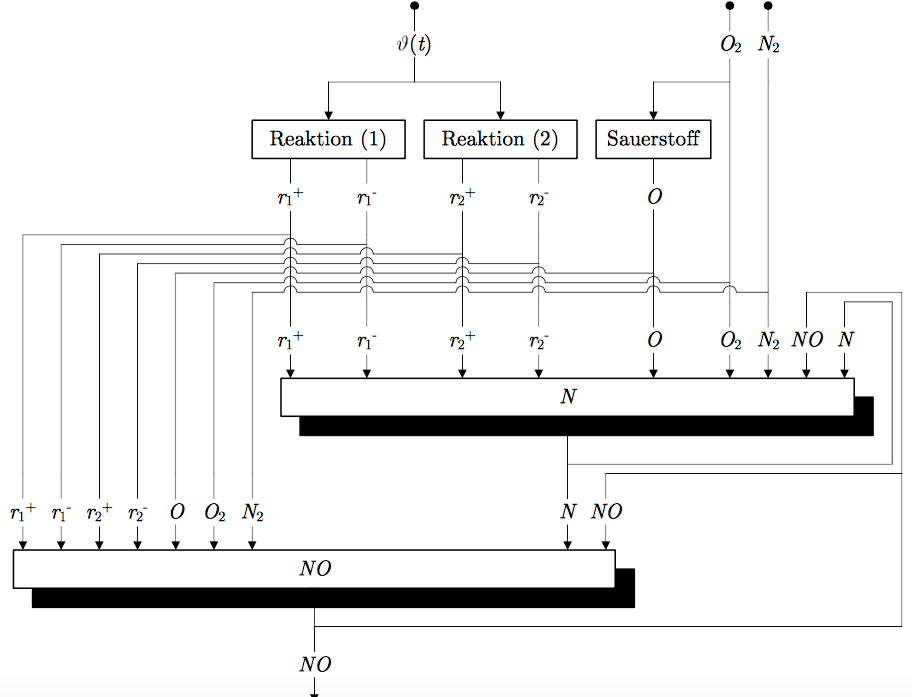
\includegraphics[width=\columnwidth]{chem_1.png}\end{center}
        \end{minipage}
		\begin{minipage}{0.5\columnwidth}
		\begin{center}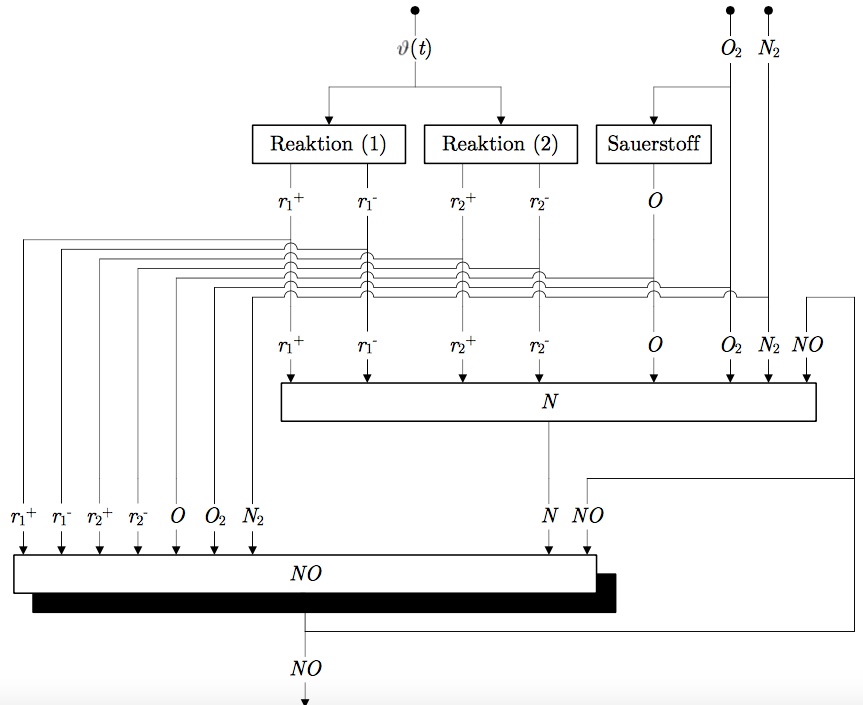
\includegraphics[width=\columnwidth]{chem_2.png}\end{center}
           \end{minipage} \\
Gegeben ist die Reaktion 
\begin{equation} N_2+O \leftrightarrow NO+N \end{equation}
\begin{equation} O_2+N \leftrightarrow NO+O \end{equation}
Mit der klassische Def. von $r_i^+$ folgt: \\
\begin{minipage}{0.4\columnwidth}
$\frac{d[NO]_1}{dt}=r_1^+[N_2][O]-r_1^-[NO][N]$\\
$\frac{d[NO]_2}{dt}=r_2^+[O_2][N]-r_2^-[NO][O]$\\
$\frac{d[N]_1}{dt}=r_1^+[N_2][O]-r_1^-[NO][N]$\\
$\frac{d[N]_2}{dt}=r_2^-[NO][O]-r_2^+[O_2][N]$\\
\end{minipage}
\begin{minipage}{0.6\columnwidth}
Durch Summieren:\\
$\frac{d[NO]}{dt}=r_1^+[N_2][O]-r_1^-[NO][N]+r_2^+[O_2][N]-r_2^-[NO][O]$\\
$\frac{d[N]}{dt}=r_1^+[N_2][O]-r_1^-[NO][N]+r_2^-[NO][O]-r_2^+[O_2][N]$\\
Falls man $\frac{d[N]}{dt}=0$ annimmt:\\
$[N]=\frac{r_1^+[N_2][O]+r_2^-[NO][O]}{r_1^-[NO]+r_2^+[O_2]}$
\end{minipage}

\subsection{Example: SCR System}
Katalytische Reduktion sehr wichtig f\"ur Diesel Motoren. Man reduziert $NO_x$ im Abgas mit $NH_3$, das durch Thermo/Hydrolyse gebildet wird. \\
\begin{minipage}{0.4\columnwidth}
		\begin{center}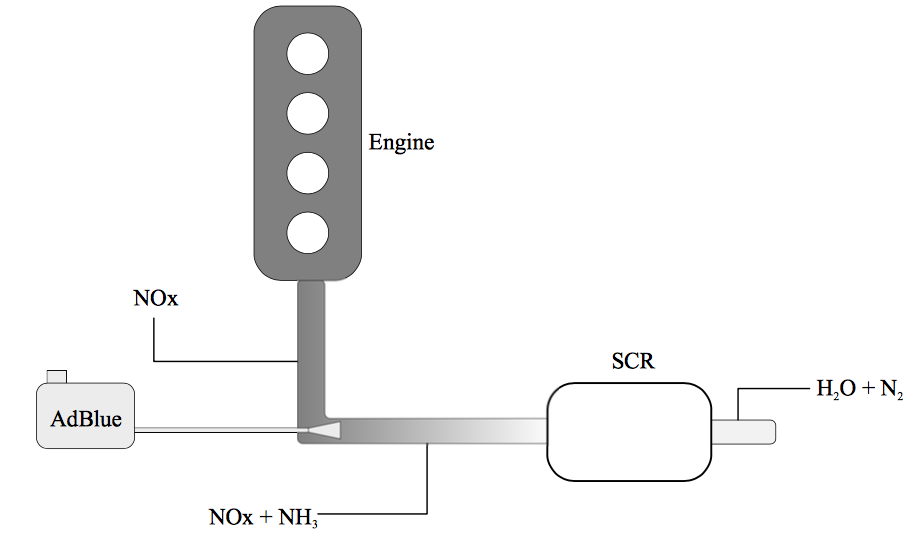
\includegraphics[width=\columnwidth]{scr_1.png}\end{center}
           \end{minipage} 
 \begin{minipage}{0.6\columnwidth}
		\begin{center}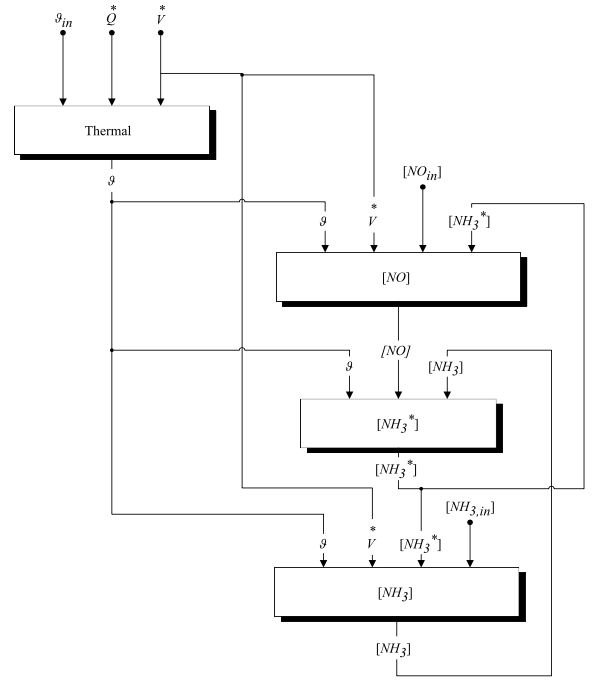
\includegraphics[width=0.5\columnwidth]{scr_2.png}\end{center}
           \end{minipage} \\
\textbf{Reaktionen:} $NH_3\leftrightarrow NH_3^*$ , $NH_3^*$: Absorbierte $NH_3$.\\
\textbf{Hauptreaktion:} $NH_3^*+NO+\frac{1}{4}O_2 \rightarrow N_2+\frac{3}{2}H_2O$, Gleichzeitig $NH_3^*+\frac{3}{4}O_2\rightarrow \frac{1}{2}N_2+\frac{3}{2}H_2O$\\
\textbf{Zustandsvariablen:} Temperatur Systems: $\vartheta$. $NO$ Gehalt: $[NO]$. $NH_3$ Gehalt: $[NH_3]$. Abs. Gehalt: $[NH_3^*]$.\\
\textbf{DGL f\"ur $NH_3^*$:} $\frac{d}{dt}[NH_3^*]=r_{ads}\cdot [NH_3]-r_{des}\cdot [NH_3^*]-r_{SCR}\cdot [NO]\cdot [NH_3^*]-r_{ox}\cdot [NH_3^*]$\\
\textbf{DGL f\"ur $NO$:} $\frac{d}{dt}n_{NO}=\dot{V}\cdot [NO_{in}]-\dot{V}\cdot [NO]-V\cdot r_{SCR}\cdot [NH_3^*]\cdot [NO]$. Man muss durch SCR Konverter Volumen dividieren: $\frac{d}{dt}[NO]=\frac{\dot{V}}{V}\cdot [NO_{in}]-\frac{\dot{V}}{V}\cdot [NO]-r_{SCR}\cdot [NH_3^*]\cdot [NO]$\\
\textbf{Arrhenius Eq. :} $r_{ads}=k_{ads}e^{-\frac{E_{ads}}{R\vartheta}}$, $r_{des}=k_{des}e^{-\frac{E_{des}}{R\vartheta}}$, $r_{SCR}=k_{SCR}e^{-\frac{E_{SCR}}{R\vartheta}}$, $r_{ox}=k_{ox}e^{-\frac{E_{ox}}{R\vartheta}}$

\subsection{Example: 3 Way Catalytic Converter}
\begin{minipage}{0.5\columnwidth}
\textbf{Reaktion:} $CO\leftrightarrow CO^*$, $O_2\rightarrow 2O^*$, $CO^*+O^*\rightarrow CO_2$\\
\textbf{Zustandsvariablen :} $[O_2]$, $[CO]$, $[O_2^*]$, $[CO^*]$\\
\textbf{DGL f\"ur $O^*$:} $\frac{d}{dt} [O^*]=2\cdot r_{O_2}[O_2]-r_{ox}[CO^*][O^*]$\\
\textbf{DGL f\"ur $CO$:} $\frac{d}{dt}n_{CO}=\dot{V}[CO_{in}]-\dot{V}[CO]-Vr_{ads}[CO]+Vr_{des}[CO^*]$. Durch $V$ dividieren liefert $\frac{d}{dt}[CO]=\frac{\dot{V}}{V}[CO_{in}]-\frac{\dot{V}}{V}[CO]-r_{ads}[CO]+r_{des}[CO^*]$
		        \end{minipage}
		\begin{minipage}{0.5\columnwidth}
		\begin{center}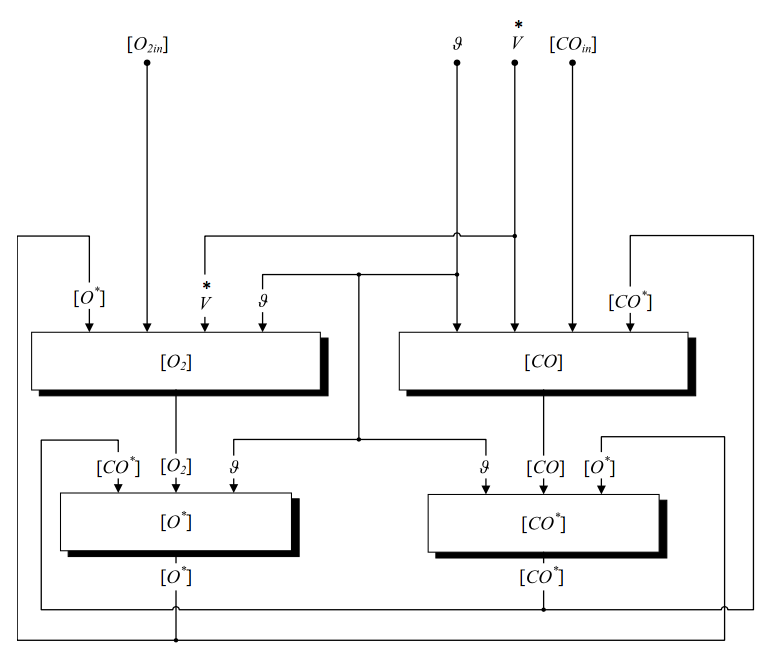
\includegraphics[width=0.67\columnwidth]{catal.png}\end{center}
           \end{minipage} \\

\subsection{Example: $CH_4$ Synthesis}
\begin{center}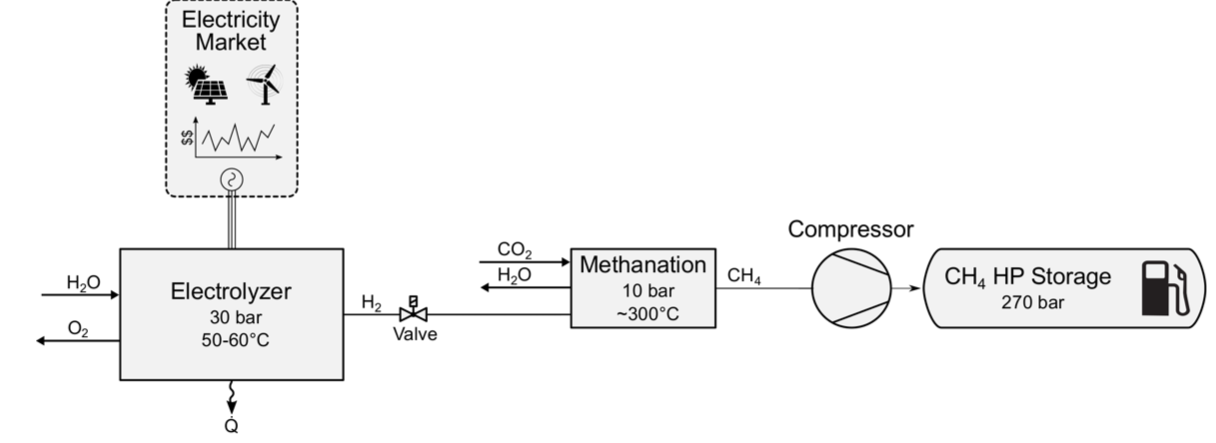
\includegraphics[width=0.65\columnwidth]{synt.png}\end{center}
Generated $CH_4$ pumped in storage tank by compressor at rate $\dot{m}_{CH_4}$. Combustion of $CH_4$ produces $CO_2$ and $H_2O$. The same amount of $CO_2$ is produced everywhere: the proces is carbon-neutral.\\
\textbf{Reaction:} $4H_2+CO_2\leftrightarrow 2H_2O+CH_4$, Forward $r_M^+$, Backward $r_M^-$. \\
\textbf{Mass-Flow:} The pressure after the valve $p_M$ is lower than the critical pressure $p_{cr}=\left( \frac{2}{\kappa_{H_2}+1} \right)^{\frac{\kappa_{H_2}}{\kappa_{H_2}-1}}\cdot p_E$. This means $\dot{m}_{H_2}=c_dA(t)\cdot \frac{p_E}{\sqrt{R\vartheta_E}}\cdot \sqrt{\kappa_{H_2}\cdot \left( \frac{2}{\kappa_{H_2}+1} \right)^{\frac{\kappa_{H_2}+1}{\kappa_{H_2}-1}}}$\\
\textbf{DGL f\"ur $H_2$:} $\frac{d[H_2]}{dt}=-4r_M^+[H_{2,M}]^4[CO_{2,M}]+4r_M^-[CH_4][H_2O]^2+\frac{\dot{m}_{H_2}(t)}{V_MM_{H_2}}$\\
\textbf{DGL f\"ur $CH_4$:} $\frac{d[H_2]}{dt}=r_M^+[H_{2,M}]^4[CO_{2,M}]-r_M^-[CH_4][H_2O]^2-\frac{\dot{m}_{CH_4}(t)}{V_MM_{CH_4}}$\\
As the throttle is isenthalpic, the temperatur of the $H_2$ after the throttle is $\vartheta_E$. Thus, the enthalpy of the $H_2$ entering the mathanation reactor is given by $\dot{H}_{H_2,M,in}=\vartheta_E\cdot c_{p,H_2}\cdot \dot{m}_{H_2}(t)$ and $\dot{H}_{H_CH_4,M,out}=\vartheta_M\cdot c_{p,CH_4}\cdot \dot{m}_{CH_4}(t)$

\subsection{Example: Continuously stirred tank reactor}

\begin{itemize}
\item The concentration [B] remains constant.
\item Dissociation $A+B\leftarrow C$ is negligible.
\item Mass $m$ and density $\rho$ are constant.
\item Perfect insulation.
\end{itemize}

\mypic{CSTR}

\begin{enumerate}
\item \begin{tabular}{ll}Input: & $\overset{\ast}{Q}(t)$ rate of heat transferred by the exchanger.\\ Outputs: & concentration C and temperature $\vartheta(t)$\end{tabular}
\item 3 Reservoirs:
\begin{itemize}
\item $n_A$ amount of species A, level variable [A]
\item $n_C$ amount of species C, level variable [C]
\item internal energy $U$, level variable $\vartheta$
\end{itemize}
\item Conservation laws:
\begin{itemize}
\item $\ddt n_A(t)=\overset{\ast}{V}[A_i(t)]-\overset{\ast}{V}[A(t)]-Vk^-[B]e^{-E/(R\vartheta(t))}[A(t)]$
\item $\ddt n_C(t)=-\overset{\ast}{V}[C(t)]+Vk^-[B]e^{-E/(R\vartheta)}[A(t)]$
\item $\ddt U(\vartheta(t),n_A(t),n_B(t),n_C(t))=\overset{\ast}{H}_i(\vartheta_i(t))-\overset{\ast}{H}_o(\vartheta(t))+\overset{\ast}{Q}(t)$
\end{itemize}
\item \begin{tabular}{l@{ = }l}$dU(\vartheta,n_A,n_B,n_C)$&$\frac{\partial U}{\partial \vartheta}d\vartheta+\frac{\partial U}{\partial n_A}dn_A+\frac{\partial U}{\partial n_B}dn_B+\frac{\partial U}{\partial n_c}dn_C$\\ &$\rho V c_vd\vartheta+H_Adn_A+H_Bdn_B+H_Cdn_C$\end{tabular}
\item \begin{tabular}{l@{ = }l}
$\tau\ddt [A(t)]$&$[A_i(t)]-(1+\tau ke^{-E/(R\vartheta(t))})[A(t)]$\\
$\tau\ddt [C(t)]$&$-[C(t)]+\tau ke^{-E/(R\vartheta(t))}[A(t)]$\\
$\tau\ddt \vartheta(t)$&$\vartheta_i(t)-\vartheta(t)+\frac{1}{\rho c_v}\frac{\overset{\ast}{Q}(t)}{\overset{\ast}{V}}+\tau H_0\frac{\kappa}{c_v\rho}e^{-E/(R\vartheta(t))}[A(t)]$
\end{tabular}
\end{enumerate}

Static behaviour of the CSTR: 

\begin{itemize}
\item $\overset{\ast}{Q}=0$
\item $\vartheta_i=const.$
\item $[A_i]=const.$
\end{itemize}

\important{$\overset{\ast}{H}_{flow}(\vartheta)+\overset{\ast}{Q}_{chem}(\vartheta)=0$}

%\important{$\overset{\ast}{H}=\overset{\ast}{m}c_p(\vartheta_i-\vartheta)$}

\important{$\overset{\ast}{Q}_{chem}(\vartheta)=H_0\frac{Vke^{-E/(R\vartheta)}}{1+\tau ke^{-E/(R\vartheta)}}[A_i]$}

\vfill
\null
\newpage

\section{Model Parametrization}

\subsection{Planning experiments}

Planning experiments is about knowing:
\begin{itemize}
\compaq
\item Choice of correct input signals
\item Choice of sensor(s) (location)
\item Measurement for (non?)linear model identification
\item Frequency content of excitation signals
\item Noise level at input and output
\item Safety issues
\end{itemize}

Experimentally obtained data may be used to:

\begin{itemize}
\ncompaq
\item Identify unknown system structures and system parameters.
\item Validate the results of the system modeling and parameter identification.
\end{itemize}

\important{Never use the same set of data for both purposes!}

\subsection{Least squares estimation}

Used to fit the parameters of a \textbf{linear} and \textbf{static} model.

\mportant{$y(k)=\mathbf{h}[\mathbf{u}(k)]^T \cdot \mathbf{\pi} + e(k)$}

\begin{itemize}
\ncompaq
\item Index of discrete time: k
\item Input vector: $\mathbf{u}(k)\in\mathbb{R}^m$
\item Output signal: $y(k)\in\mathbb{R}$
\item Vector of unknown parameter: $\mathbf{\pi}\in\mathbb{R}^q$
\item Regressor: $\mathbf{h[.]}\in\mathbb{R}^q$
\item r = number of measurements taken
\item Typically $r\gg q$
\end{itemize}

y should be chosen such that it contains the measurement with the most significant error which we want to minimise.

We want to minimise the following equation:

\mportant{$\epsilon = \tilde{e}^T \cdot W \cdot \tilde{e}$}

Where $W = \text{diag} (w_1, ..., w_n)$ is a symmetric, positive definite weighting matrix.
If all measurements are equally reliable, one can choose $W=\mathbb{I}$.

\important{$\pi_{LS}=[H^T\cdot W\cdot H]^{-1}H^T\cdot W\cdot \tilde{y}$}

\mypic{LSQ}

Where H must have full column rank \dahe all q parameters ($\pi_1,\pi_2,\ldots,\pi_q)$ are required to explain the data.

\importname{Moore-Penrose inverse}{$M^\dagger = (M^T\cdot M)^{-1}\cdot M^T$}

Where $M\in\mathbb{R}^{r\times q},\ r>q,\ \text{rank}\{M\}=q$.

\finn

If the error e is an \textbf{uncorrelated white noise signal} with \textbf{mean value 0} and \textbf{variance $\sigma$}.

Then:
\begin{itemize}
\ncompaq
\item expected value: $\expe{\pi_LS}=\pi_{true}$
\item covariance matrix: $\sum=\sigma^2\cdot(H^T\cdot W\cdot H)^{-1}$
\end{itemize}

\important{$\A^{-1}=\begin{bmatrix}a&b\\c&d\end{bmatrix}^{-1}=\frac{1}{ad-bc}\begin{bmatrix}d&-b\\-c&a\end{bmatrix}$}

\subsubsection{Examples: Straight line and parabola}
\begin{itemize}
\item \textbf{Straight line}:\\
$\hat{e}=\hat{y}-(ax+b)=\hat{y}- \begin{pmatrix} x&1 \end{pmatrix} \cdot \begin{pmatrix} a\\ b\end{pmatrix}=\hat{y}-H\pi$
\item \textbf{Parabola}:\\
$\hat{e}=\hat{y}-(ax^2+bx+c)=\hat{y}- \begin{pmatrix} x^2&x&1 \end{pmatrix} \cdot \begin{pmatrix} a\\ b \\ c\end{pmatrix}=\hat{y}-H\pi$
\end{itemize}

\subsubsection{Example: Least Squares on a DC-Motor}
We have conducted two steady-state measurements of $u_i,T_{l,i},\omega_i,I_i$ without significant measurement errors.
We are now looking for $\kappa$ and $d$ while we know that $R=1$.
Therefore the vector of unknown parameters is $\pi=\begin{pmatrix} \kappa \\d\end{pmatrix}$ and the weighting matrix $W=\mathbb{I}$.\\

Based on the equations:\\
$L\frac{d}{dt}I(t)=u(t)-RI(t)-\kappa \omega(t)$\\
$\Theta \frac{d}{dt}\omega(t)=\kappa I(t)-T_l(t)-d\omega(t)$\\
We rewrite the equations according to what we are looking for:
\begin{align*}
\kappa\omega_i =&u_i-R_iI_i\\
\kappa I_i-d\omega_i =&T_{l,i}
\end{align*}
The error can be written as:
\begin{align*}
\tilde e =&\tilde y - H \cdot \pi\\
\tilde e =&\begin{pmatrix} u_1-RI_1\\T_{l,1}\\u_2-RI_2\\T_{l,2}\end{pmatrix}-\begin{pmatrix} \omega_1&0\\I_1 &-\omega_1\\ \omega_2&0\\I_2 &-\omega_2\end{pmatrix}\cdot\begin{pmatrix} \kappa \\d\end{pmatrix}
\end{align*}

%\textbf{Falls R unbekannt und d bekannt:} $\pi=\begin{pmatrix} \kappa \\ R\end{pmatrix}$, $y=\begin{pmatrix} u_1\\T_{l,1}+d\cdot \omega_1\\u_2\\T_{l,2}+d\cdot \omega_2\end{pmatrix}$, $H=\begin{pmatrix} \omega_1 & I_1\\ I_1&0\\ \omega_2 & I_2\\ I_2 & 0 \end{pmatrix}$

\vfill
\null
\columnbreak

\subsection{Iterative Least Squares}

\mportant{$\pi_{LS}=[H^T\cdot W\cdot H]^{-1}H^T\cdot W\cdot \tilde{y}$}

Motivation: If an additional measurement is taken, we don't want to recompute the inverse $[H^T\cdot W\cdot H]^{-1}$ 

\mportname{Iterative approach}{$\pi_{LS (r+1)}=f(\pi_{LS (r)},y_{(r+1)})$}

\begin{enumerate}
\ncompaq
\item \textbf{Start:} $\pi_{LS}=[H^T\cdot W\cdot H]^{-1}H^T\cdot W\cdot \tilde{y}$
\item \textbf{Simplification:} $W=I\quad\rightarrow\quad \pi_{LS}=[H^T\cdot H]^{-1}\cdot\tilde{y}$
\item \textbf{Formulate matrix products as sums:}

$\pi_{LS (r)}=\left[\sum\limits_{k=1}^r h_{(k)} \cdot h^T_{(k)} \right]^{-1} \cdot \sum\limits_{k=1}^r h_{(k)} \cdot y_{(k)}$
\item \textbf{Use matrix inversion Lemma}

Notation: $\Omega_{(r)} = \left[\sum\limits_{k=1}^r h_{(k)} \cdot h^T _{(k)} \right]^{-1}$

$\Omega_{(r+1)} = \left[\sum\limits_{k=1}^r h_{(k)} \cdot h^T_{(k)} + h_{(r+1)} \cdot h^T_{(r+1)} \right]^{-1}$

\dahe Matrix inversion Lemma leads to:

\item \textbf{How to recursively compute the estimate:}

\mportant{$\pi_{LS (r+1)}=\Omega_{(r)} \cdot \sum\limits_{k=1}^{r} h_{(k)} y_{(k)}$}

\mportant{$\pi_{LS (r+1)} =\Omega_{(r+1)} \cdot \sum\limits_{k=1}^{r+1} h_{(k)} y_{(k)}$}

\importabflex{l}{$\pi_{LS (r+1)}=\pi_{LS (r)}+$\\
$+\underbrace{\frac{1}{1+c_{(r+1)}}\Omega_{(r)}h_{(r+1)}}_A\underbrace{\left(y_{(r+1)}-h^T_{(r+1)}\pi_{LS(r)}\right)}_B$\\
$\Omega_{(r+1)} =\Omega_{(r)}-$\\
$-\frac{1}{1+c_{(r+1)}} \cdot \Omega_{(r)} \cdot h_{(r+1)} \cdot h^T_{(r+1)} \cdot \Omega_{(r)}$\\
where $c_{(r+1)} = h^T_{(r+1)} \cdot \Omega_{(r)} \cdot h_{(r+1)}$
}

A: Indicates the correction direction. \\
B: Innovation term or prediction error.
\end{enumerate}

\subsubsection{Matrix inversion Lemma}

Suppose $M\in\mathbb{R}^{n\times n}$ regular $(\det(M)\neq 0)$ \\
$v\in\mathbb{R}^n:\quad 1+v^T\cdot M^{-1}\cdot v \neq 0$ \\
$[M+v\cdot v^T]^{-1}=M^{-1}-\frac{1}{1+v^T\cdot M^{-1}\cdot v}\cdot M^{-1}\cdot v\cdot v^T\cdot M^{-1}$

\subsection{Exponential Forgetting}

\mportant{$\epsilon_{(r)} = \sum\limits_{k=1}^r \lambda^{r-k} [y_{(k)} - h^T_{(k)} \cdot \pi_{LS (k)} ]^2, \quad \lambda<1$}

\small
\importabflex{l}{
\vtabfill \\
$\pi_{LS (r+1)} = \pi_{LS (r)} + \frac{1}{\lambda+c_{(r+1)}} \Omega_{(r)} h_{(r+1)} \left[y_{(r+1)} - h^T_{(r+1)} \pi_{LS (r)} \right]$\\
$\Omega_{(r+1)} = \frac{1}{\lambda}\Omega_{(r)} \left[\mathbb{I} - \frac{1}{\lambda+c_{(r+1)}}h_{(r+1)}h^T_{(r+1)}\Omega_{(r)}\right]$
}\normalsize

\subsection{Simplified Recursive LS Algorithm}
Each new prediction error $\epsilon_{(r+1)} = y_{(r+1)} - h^T_{(r+1)} \cdot \pi_{(r)}$ contains new information on $\pi$ only in the direction of $h_{(r+1)}$. Therefore $\pi_{(r+1)}$ is sought, which requires the smallest possible change $\pi_{(r+1)}-\pi_{(r)}$ to explain the new observation.\\
Cost function to minimize:

\mportant{$J(\pi)=\onha\cdot[\pi_{(r+1)}-\pi_{(r)}]^T \cdot (\pi_{(r+1)}-\pi_{(r)}) + \mu\cdot [y_{(r+1)}-h^T_{(r+1)}\cdot\pi_{(r+1)}]$}

Necessary conditions for the minimum:

\mportant{$\frac{\partial J}{\partial\pi_{(r+1)}}=0\qquad \frac{\partial J}{\partial \mu}=0$}

Solution:

\important{$\pi_{(r+1)}=\pi_{(r)}+\frac{h_{(r+1)}}{h^t_{(r+1)}\cdot h_{(r+1)}}\cdot[y_{(r+1)}-h^T_{(r+1)}\cdot\pi_{(r)}]$}

Modification with $0<\gamma<2$ for convergence, $0<\lambda<1$ for forgetting

\important{$\pi_{(r+1)}=\pi_{(r)}+\frac{\gamma \cdot h_{(r+1)}}{\lambda+h^t_{(r+1)}\cdot h_{(r+1)}}\cdot[y_{(r+1)}-h^T_{(r+1)}\cdot\pi_{(r)}]$}

\begin{itemize}
\item Kaczmarz' projection algorithm requires less computational effort.
\item It converges much slower than regular LS algorithms.
\end{itemize}

\vfill
\null
%\columnbreak
\newpage

\section{Analysis of Linear Systems}

\subsection{Normalization}

\mportant{$\bar{x}_i(t)=\frac{x_i(t)}{x_{i,0}},\quad \bar{u}_j(t)=\frac{u_j(t)}{u_{j,0}},\quad \bar{y}_k(t)=\frac{y_k(t)}{y_{k,0}}$}

With the scaling factors: $x_{i,0},u_{j,0},y_{k,0}$. \\
The normalized variables $\bar{x}_i(t),\ \bar{u}_j(t)$ and $\bar{y}_k(t)$ have \textbf{no physical units} and are \textbf{close to 1}.

\mportant{$x=T\cdot\bar{x},\quad T=\text{diag}\{x_{1,0},\ldots,x_{n,0}\}$}

Where T is the \textbf{similarity transform matrix}.

After transforming the system has the form:

\mportabflex{r@{ = }l}{
$\ddt \bar{x}(t)$&$\dot{\bar{x}}(t)=f_0(\bar{x}(t),\bar{u}(t),t)$\\
$\bar{y}(t)$&$g_0(\bar{x}(t),\bar{u}(t),t)$
}

Where $\bar{x}(t)\in\mathbb{R}^n,\ \bar{u}(t)\in\mathbb{R}^m,\ \bar{y}(t)\in\mathbb{R}^p$.

\subsection{Linearisation}

\mportname{operating point $\{x_0,u_0\}$}{$B_r:=\{x\in\mathbb{R}^n\ |\ ||x-x_0||^2+||u-u_0||^2\leq r\}$}

\mportname{equilibrium point $\{x_e,u_x\}$}{$B_r:=\{x\in\mathbb{R}^n\  |\ ||x-x_e||^2+||u-u_e||^2\leq r\}$}

Around a chosen equilibrium point $\{x_e,u_e\},\ f_o(x_e,u_e,t)=0$.

\mypic{Linearization}

$\dot{x}=f(x,u)=\textcolor{red}{f(x_0,u_0)}+\textcolor{blue}{\left.\frac{\partial f}{\partial x}\right|_{x_0,u_0}}\underbrace{(x-x_0)}_{\delta x}+$ \\
$\textcolor{blue}{\left.\frac{\partial f}{\partial u}\right|_{x_0,u_0}}\underbrace{(u-u_0)}_{\delta u}+\frac{1}{2}\left.\frac{\partial^2 f}{\partial x^2}\right|_{x_0,u_0}(x-x_0)^2+\ldots$

\mportabflex{r@{ = }l}{
$\tilde{x}(t)$&$x(t)-x_e$\\
$\tilde{u}(t)$&$u(t)-u_e$\\
$\tilde{y}(t)$&$y(t)-g_0(x_e,u_e,t)$\\
$\ddt \tilde{x}(t)$&$\tilde{f}_0(\tilde{x}(t),\tilde{u}(t),t)$\\
$\tilde{y}(t)$&$\tilde{g}_0(\tilde{x}(t),\tilde{u}(t),t)$
}

Where $\tilde{f}_0(0,0,t)=0$.

Introduction of new variables: 

\mportabflex{l@{ = }l}{
$x_i(t)$&$x_e+\delta x_i(t)$ with $|\delta x_i|\ll 1$\\
$u_i(t)$&$u_e+\delta u_i(t)$ with $|\delta u_i|\ll 1$\\
$y_i(t)$&$y_e+\delta y_i(t)$ with $|\delta y_i|\ll 1$
}

Taylor series neglecting all terms of second and higher order yields:

\mportabflex{r@{ = }l}{
$\ddt \delta x(t)$&$\left.\frac{\partial f_0}{\partial x}\right|_{x_e,u_e}\delta x(t)+\left.\frac{\partial f_0}{\partial u}\right|_{x_e,u_e}\delta u(t)$\\
$\delta y(t)$&$\left.\frac{\partial g_0}{\partial x}\right|_{x_e,u_e}\delta x(t)+\left.\frac{\partial g_0}{\partial u}\right|_{x_e,u_e}\delta u(t)$
}

\importabflex{r@{ = }c@{ + }l}{
$\ddt x(t)$&$Ax(t)$&$Bu(t)$\\
$y(t)$&$Cx(t)$&$Du(t)$
}

\important{$e^{At}=\mathbb{I}+\frac{1}{1!}At+\frac{1}{2!}(At)^2+\cdots+\frac{1}{n!}(At)^n+\cdots$}

\begin{itemize}
\item$\frac{de^{At}}{dt}=Ae^{At}=e^{At}A$
\item $e^A\cdot e^B\neq e^{A+B}$
\item If A and B commute: $e^A+e^B=e^{A+B}$
\end{itemize}

Solving the differential equation for x yields:

\mportant{$x(t)=e^{At}x(0)+\int_0^t e^{At-\sigma}B u(\sigma)d\sigma$}

\subsection{Stabilty}

\subsubsection{Lyapunov Stability}

\begin{itemize}
\item asymptotically stable if $\lim\limits_{t\rightarrow\infty}||x(t)||=0$
\item stable if $||x(t)||<\infty\ \forall\ t\in[0,\infty]$
\item unstable if $\lim\limits_{t\rightarrow\infty}||x(t)||=\infty$
\end{itemize}

\subsubsection{Eigenvalues}

\important{$Av_i=\lambda_i v_i$}

Where eigenvectors $v_i$ and eigenvalues $\lambda_i$.

\mportant{$T=[v_1,\cdots, v_n]\rightarrow AT=T\Lambda \Rightarrow T^{-1}AT=\Lambda$}

$\Lambda =\begin{bmatrix}\lambda_1&0&\cdots&0\\\vdots&&&\vdots\\\vdots&&&\vdots\\0&\cdots&0&\lambda_n\end{bmatrix}$

\begin{itemize}
\item multiplicity of $\lambda_i$=$r_i$
\item rank loss of $[\lambda_i-A]:\ \rho_i$
\end{itemize}

\hlyellow{Stability of linear systems:}
\begin{itemize}
\item All $\Re(\lambda_i)<0\ \forall\ i\Rightarrow\ $ system is asymptotically stable
\item $\Re(\lambda_i)\leq0\ \forall\ i\Rightarrow$ system is Lyapunov stable
\item $\Re(\lambda_i)>0\Rightarrow$ system is unstable
\end{itemize}

\hlgreen{Conclusions on nonlinear systems:}
\begin{itemize}
\item Linear system is asymptotically stable \\ \dahe nonlinear system is (locally) asymptotically stable.
\item Linear system is unstable \\ \dahe nonlinear system is (locally) unstable.
\item Linear system is stable \\ \dahe no conclusions on the nonlinear system.
\end{itemize}

\subsection{Continuous time transition matrix}

\mportant{$\Phi(t)=e^{At}=I+At+\frac{(At)^2}{2!}+\cdots+\frac{(At)^n}{n!}+\cdots$}

\important{$x(t)=\Phi(t)x(0)+\int_0^t\Phi(t-\sigma)Bu(\sigma)d\sigma$}

For stability analysis $u=0$ and $x(t)=\Phi(t)x(0)$!

\subsection{Reachability}

\important{$x(\tau)=e^{A\tau}\int_0^\tau e^{-A\sigma}Bu(\sigma)d\sigma$}

All the states that can be reached within $\tau$.

\important{$\mathcal{R}_n=\begin{bmatrix}B&AB&A^2B&A^3B&\cdots&A^{n-1}B\end{bmatrix}$}

If $\text{rank}(R_n)=n$ the system is reachable for all $x(0)$.

\subsection{Controllability}

Is it possible to reconstruct $x(0)$ using the output signal $y(t)$ only?

\important{$\mathcal{O}_n=\begin{bmatrix}C\\CA\\\vdots\\CA^{n-1}\end{bmatrix}$}

If $\text{rank}(\mathcal{O}_n=n)$ the system is observable.

\vfill

\section{Balanced Realization and Order Reduction}

The Gramian matrices only exist if the system is asymptotically stable!

\importname{Controllability Gramian}{$W_R=\int_0^\infty e^{A\sigma}BB^Te^{A^T\sigma}d\sigma$}

The closer $W_R$ is to a singular matrix ($\det$ close to 0), the less controllable the system will be.

\importname{Observability Gramian}{$W_O=\int_0^\infty e^{A^T\sigma}C^TCe^{A\sigma}d\sigma$}

The closer $W_O$ is to a singular matrix ($\det$ close to 0), the less observable the system will be.

\dahe Check which element in the Gramian matrix is the smallest and reduce that state.

\columnbreak

\subsection{Hurwitz systems}

\importname{Hurwitz stable}{All EV have strictly negative real parts.}

Then the Gramian matrices are the solutions of the two Lyapunov equations:

\mportable{
$AW_R+W_RA^T$&$=-BB^T$\\
$A^TW_O+W_OA$&$=-C^TC$
}

If $W_R$ is symmetric:

\mportant{
$W_R A^T = (A W_R^T)^T = (A W_R)^T$
}

%\vfill
%\null
%\columnbreak
%\section{Order reduction}

Assume that the last $\nu$ elements $\sigma_j$ with $j=n-\nu+1$ are substantially smaller than the other first $n-\nu$ elements $\sigma_i$ with $i=1,\ldots, n-\nu$. Then the contribution of the last $\nu$ balanced modes may be negleted.

\finn

Bad idea: Simply delete those system parts with minor contribution.

\finn

Good idea: Find a coordinate transformation $T\cdot x_b=x$ that yields a system with diagonal Gramians.

\begin{itemize}
\item Calculate $W_R,W_O$ by solving the Lyapunov equations.
\item Find the coordinate transformation such that $W_R,W_O=$diag$(w_i)$ and $W_R=W_O$.
\item \mportable{
$\tilde{A}$&$=T^{-1}AT$\\
$\tilde{B}$&$=T^{-1}B$\\
$\tilde{C}$&$=CT$\\
$\tilde{D}$&$=D$
}
\end{itemize}

\textcolor{red}{Normalize the system in advance!}

\begin{enumerate}
\ncompaq
\item System partitioning
Last $\nu$ elements $\sigma_j$ are substantially smaller than the other first.

\mportabflex{c@{ = }rr}{
$\ddt\begin{bmatrix}x_1(t)\\x_2(t)\end{bmatrix}$&$\begin{bmatrix}A_{1,1}&A_{1,2}\\A_{2,1}&A_{2,2}\end{bmatrix}\begin{bmatrix}x_1(t)\\x_2(t)\end{bmatrix}$&$+\begin{bmatrix}B_1\\B_2\end{bmatrix}$\\
$y(t)$&$\begin{bmatrix}C_1&C_2\end{bmatrix}\begin{bmatrix}x_1(t)\\x_2(t)\end{bmatrix}$&$+Du(t)$
}
Where $x_1\in\mathbb{R}^{n-\nu}$ and $x_2\in\mathbb{R}^\nu$.
\item Reduction
\mportabflex{c@{ = }rr}{
$\ddt x_1(t)$&$A_{11}x_1(t)$&$+B_1u(t)$\\
$y(t)$&$C_1x_1(t)$&$+Du(t)$
}

This yields good agreement in the frequency domain, but in general the DC gains and the reduced order system will be different!

\end{enumerate}

\subsubsection{Calculation of the DC-Gain}

\mportant{$P(s)=C(sI-A)^{-1}B+D$}

\importname{DC-Gain}{$P(s=0)=CA^{-1}B+D$}

\subsection{Singular perturbation}

Neglect the dynamics of the last $\nu$ states but not their DC contributions. \dahe DC gain does not change.

\mportant{$\ddt x_2(t)=0\rightarrow \textcolor{blue}{x_2(t)=-A_{2,2}^{-1}[A_{2,1}x_1(t)+B_2u(t)]}$

\mportabflex{c@{ = }rr}{
$\ddt x_1(t)$&$[A_{1,1}-\textcolor{blue}{A_{1,2}A_{2,2}^{-1}A_{2,1}}]x_1(t)$&$+[B_1\textcolor{blue}{-A_{1,2}A_{2,2}^{-1}B_2}]u(t)$\\
$y(t)$&$[C_1-\textcolor{blue}{C_2A_{2,2}^{-1}A_{2,1}}]x_1(t)$&$+[D\textcolor{blue}{-C_2A_{2,2}^{-1}B_2}]u(t)$
}
}

This is always possible if the original system was asymptotically stable.

\subsection{Example: Equation of eliminated state}

$\dot{\tilde{x}}_1=-1.9\tilde{x}_1-0.06\tilde{x}_2-0.08\tilde{x}_3+0.41\tilde{u}_4$

$\ddt\tilde{x}_1=0\Rightarrow \tilde{x}_1=-0.03\tilde{x}_2-0.04\tilde{x}_3+0.22\tilde{u}$

\vfill
\null
\columnbreak

\section{Zero Dynamics}

\mportabflex{ll@{ = }l@{ + }l}{
$\ddt x(t)=$&$\dot{x}(t)$&$Ax(t)$&$Bu(t)$\\
&$y(t)$&$Cx(t)$&$Du(t)$
}

\importname{Transfer function}{$P(s)=C\dot[sI-A]^{-1}\cdot B+D$}

\mportant{$P(s)=\frac{Y(s)}{U(s)}=\textcolor{red}{k}\frac{s^{n-r}+\textcolor{orange}{b_{n-r-1}}s^{n-r-1}+\cdots+\textcolor{orange}{b_1} s+\textcolor{orange}{b_0}}{s^n+\textcolor{blue}{a_{n-1}}s^{n-1}+\textcolor{blue}{a_{n-2}}s^{n-2}+\cdots+\textcolor{blue}{a_2}s^2+\textcolor{blue}{a_1}s+\textcolor{blue}{a_0}}$}
\begin{itemize}
\ncompaq
\item The order of the highest power is \textcolor{blue}{$n$}.
\item Input gain: \textcolor{red}{k}
\item The relative degree $r$
\end{itemize}

\subsubsection{State-Space Representation}

\mportabflex{l@{ = }l}{
$\ddt x(t)$&$\begin{bmatrix}0&1&0&\cdots&0\\0&0&1&\cdots&0\\\vdots&\vdots&\vdots&\cdot&\vdots\\0&0&0&\cdots&1\\-\textcolor{blue}{a_0}&-\textcolor{blue}{a_1}&-\textcolor{blue}{a_2}&\cdots&-\textcolor{blue}{a_{n-1}}\end{bmatrix}x(t)+\begin{bmatrix}0\\0\\\vdots\\0\\\textcolor{red}{k}\end{bmatrix}u(t)$\\
$y(t)$&$\begin{bmatrix}\textcolor{orange}{b_0}&\cdots&\textcolor{orange}{b_{n-r-1}}&\textcolor{orange}{1}&1&0\cdots&0\end{bmatrix}x(t)=\textcolor{orange}{C}x(t)$
}

This is the controller canonical form.

\subsection{Zero Dynamics - Definition}

The zero dynamics of a system correspond to its behaviour for special non-zero inputs $u^\ast(t)$ and initial conditions $x^\ast$ for which $y(t)$ is identical to zero for i finite interval.

\begin{itemize}
\ncompaq
\item Study the influence of zeros on the dynamics of the system.
\item Study the internal dynamics / Analyse the stability of system states which are not directly controlled by the input.
\end{itemize}

The relative degree r is the \textbf{number of differentiations needed} to have the input $u(t)$ explicitly appear in the output $y^{(r)}(t)$

\mportabflex{lll}{
$y(t)$&=&$Cx(t)$\\
$\dot{y}(t)$&=&$C\dot{x}(t)=CAx(t)+CBu(t)=CAx(t)$\\
$\ddot{y}(t)$&=&$CA^2x(t)+CABu(t)=CA^2x(t)$\\
&$\vdots$&\\
$y^{(r-1)}(t)$&=&$CA^{r-1}x(t)+CA^{r-2}Bu(t)=CA^{r-1}x(t)$\\
$y^{(r)}(t)$&=&$CA^rx(t)+\textcolor{red}{k}u(t)$
}

Then we transform coordinates (with $\Phi$) as follows:

\mportabflex{rll}{
\hlcyan{$z_1$}=$y$&$=Cx$&$=[\textcolor{orange}{b_0}x_1+\textcolor{orange}{b_1}x_2+...+\textcolor{orange}{b_{n-r-1}}x_{n-r}+x_{n-r+1}]$\\
$z_2=\dot{y}$&$=CAx$&$=[\textcolor{orange}{b_0}x_2+\textcolor{orange}{b_1}x_3+...+\textcolor{orange}{b_{n-r-1}}x_{n-r+1}+x_{n-r+2}]$\\
&$\vdots$&$\vdots$\\
$z_r=y^{(r-1)}$&$=CA^{r-1}x$&$=[\textcolor{orange}{b_0}x_r+\textcolor{orange}{b_1}x_{r+1}+...+\textcolor{orange}{b_{n-r-1}}x_{n-1}+x_n]$\\
$y^{(r)}$&$=CA^rx+\textcolor{red}{k}u$&$=[\textcolor{orange}{b_0}x_{r+1}+\textcolor{orange}{b_1}x_{r+2}+...+\textcolor{orange}{b_{n-r}}x_n+\textcolor{blue}{\dot{x}_n}]$
}

The remaining n-r coordinates are chosen such that the transformation $\Phi$ is regular and such that their derivatives dont depend on u.

\mportant{$\begin{matrix}z_{r+1}&=&x_1\\z_{r+2}&=&x_2\\&\vdots&\\z_n&=&x_n-r\end{matrix}$}

Then the vector z is partitioned into subvectors:

\mportant{$z=\begin{bmatrix}\zeta\\\eta\end{bmatrix},\quad \zeta=\begin{bmatrix}z_1\\\vdots\\z_r\end{bmatrix},\quad\eta=\begin{bmatrix}z_{r+1}\\\vdots\\z_n\end{bmatrix}$}

New form of the system:

\tiny
$\begin{bmatrix}\dot{\zeta}\\\dot{\eta}\end{bmatrix}=
\left[\begin{tabular}{ccccc|ccccc}
	0&1&0&$\cdot$&0&0&$\cdot$&$\cdot$&$\cdot$&0\\
	0&0&1&$\cdot$&0&0&$\cdot$&$\cdot$&$\cdot$&0\\
	0&$\cdot$&$\cdot$&0&1&0&$\cdot$&$\cdot$&$\cdot$&0\\
	-&-&$r^T$&-&-&-&-&$s^T$&-&-\\
	\hline
	0&$\cdot$&$\cdot$&$\cdot$&0&0&1&0&$\cdot$&0\\
	0&$\cdot$&$\cdot$&$\cdot$&0&0&0&1&$\cdot$&0\\
	0&$\cdot$&$\cdot$&$\cdot$&0&0&$\cdot$&$\cdot$&0&1\\
	-&-&$p^T$&-&-&-&-&$q^T$&-&-
	\end{tabular}\right]\begin{bmatrix}\zeta\\\eta\end{bmatrix}+\left[\begin{tabular}{c}0\\ $\cdot$\\0\\k\\\hline\\0\\ $\cdot$ \\ $\cdot$ \\0\end{tabular}\right]u$
\normalsize

\hlcyan{and $y=z_1$}

The precise form of the vectors $r^T$ and $s^T$ is not important.
Furthermore $p^T=\begin{bmatrix}1&0&\cdots&0\end{bmatrix}$ and $q^T=\begin{bmatrix}-b_0&-b_1&\cdots&-b_{n-r-2}&-b_{n-r-1}\end{bmatrix}$.

To achieve a vanishing output we choose:

\mportant{$\zeta^\ast = 0,\quad u^\ast(t)=-\frac{1}{k}s^T\eta^\ast(t)$}

Where $\eta_0^\ast\neq 0$ can be chosen arbitrarily.

Then the internal states (zero dynamic states) evolve as follows:

\mportant{$\ddt\eta(t)=\begin{bmatrix}0&1&0&\cdots&0\\0&0&1&\cdots&0\\0&\cdots&\cdots&0&1\\-&-&q^T&-&-\end{bmatrix}\eta^\ast(t)=Q\eta^\ast(t)$}

Where $\eta^\ast(0)=\eta_0^\ast$ and $q^T=\begin{bmatrix}-b_0&-b_1&\cdots&-b_{n-r-2}&-b_{n-r-1}\end{bmatrix}$ as above.

\vfill
\null
\newpage

\subsection{Minimum Phase}

If the matrix $Q$ is asymptotically stable the system is \textbf{minimum phase}.

As soon as there is a zero with a positive real part:

\begin{itemize}
\ncompaq
\item The system is non-minimum phase.
\item The system has unstable zero dynamics.
\item its internal states $\eta$ can diverge without $y(t)$ being affected.
\end{itemize}

Consequences:

\begin{itemize}
\ncompaq
\item The input $u(t)$ may not be chosen such that $y(t)$ is (almost) zero before the states $\eta$ are (almost) zero.
\item Feedback control is more difficult to design.
\item This imposes a constraint on the bandwidth of the closed-loop system: The controller must be significantly slower than the slowest non-minimumphase zero.
\end{itemize}

\mportabflex{l@{ = }l}{
$\dot{z}_n$&$\dot{x}_{n-r}$\\
&$x_{n-r+1}$\\
&$z_1-b_0x_1\ldots-b_{n-r-1}x_{n-r}$\\
&$z_1-b_0z_{r+1}\ldots -b_{n-r-1}z_n$\\
&$z_1+q^T\eta$
}

Therefore the EV of Q coincide with the transmission zeros of the original system and with the roots of the numerator of its transfer function.

\mypic{ZeroDynamics}

\subsection{Summary of the procedure}

\begin{enumerate}
\ncompaq
\item Convert the plant's transfer function into a state-space controller canonical form.
\item Find r and do the coordinate transform sucht that $z=\Phi^{-1}\cdot x$
\item Find the transformation matrices $\Phi^{-1}$ and then compute $\Phi$
\item Build a new state-space representation in $z=\begin{bmatrix}\zeta\\\eta\end{bmatrix}$.
\item Study the submatrix $Q$ of $\tilde{A}=\Phi^{-1}A\Phi$ corresponding to the zero-dynamics vector $\eta$. 
\end{enumerate}

\subsection{Example: Small SISO System}

\begin{enumerate}[leftmargin=*]
\ncompaq
\item Transfer function \dahe state-space controller canonical form
\mportant{$P(s)=\frac{Y(s)}{U(s)}=k\frac{b_1s+b_0}{a_3s^3+a_2s^2+a_1s+a_0}$}
\mportabflex{rrr}{$\ddt x(t)$&$=\begin{bmatrix}0&1&0&0\\0&0&1&0\\0&0&0&1\\-a_0&-a_1&-a_2&-a_3\end{bmatrix}\cdot x(t)$&$+\begin{bmatrix}0\\0\\0\\k\end{bmatrix}\cdot u(t)$\\
$y(t)=$&$\begin{bmatrix}b_0&b_1&1&0\end{bmatrix}\cdot x(t)$&$+[0]\cdot u(t)$
}
\item Coordinate transformation

$r=2\Longrightarrow$

\mportable{
$y(t)$&$=b_0x_1(t)+b_1x_2(t)+x_3(t)$\\
$\dot{y}(t)$&$=b_0x_2(t)+b_1x_3(t)+x_4(t)$\\
$\ddot{y}(t)$&$-a_0x_1(t)-a_1x_2(t)+(b_0-a_2)x_3(t)+$\\
&$+(b_1-a_3)x_4(t)+\textcolor{blue}{ku(t)}$
}

The coordinate transform $z=\Phi^{-1}\cdot x$ has the form:

\mportabflex{c@{=}cl}{
$z_1$&$y$&$=b_0x_1+b_1x_2+x_3$\\
$z_2$&$\dot{y}$&$=b_0x_2+b_1x_3+x_4$\\
$z_3$&$x_1$\\
$z_4$&$x_2$
}
\item Find $\Phi^{-1}:\ z=\Phi^{-1}\cdot x$ and then compute $\Phi$

\hlpink{Alternatively solve $z=\Phi^{-1}\cdot x$ for $x_i(z_i)$ to get $\Phi$. }

\mportant{$\Phi^{-1}=\begin{bmatrix}b_0&b_1&1&0\\0&b_0&b_1&1\\1&0&0&0\\0&1&0&0\end{bmatrix}$}

\mportant{$\Phi=\begin{bmatrix}0&0&1&0\\0&0&0&1\\1&0&-b_0&-b_1\\-b_1&1&b_0b_1&b_1^2-b_0\end{bmatrix}$}

\item New state-space representation in $z=\begin{bmatrix}\zeta\\ \eta\end{bmatrix}$

\mportant{$\zeta=\begin{bmatrix}z_1\\z_1\end{bmatrix},\ \eta=\begin{bmatrix}z_3\\z_4\end{bmatrix}$}

\mportable{
$\ddt z(t)$&$=\Phi^{-1}A\Phi z(t)+\Phi^{-1}Bu(t),\ y(t)=C\Phi z(t)$\\
$\ddt \begin{bmatrix}\zeta_1(t)\\\zeta_2(t)\\\zeta_3(t)\\\zeta_4(t)\end{bmatrix}$&$=\begin{bmatrix}0&1&0&0\\r_1&r_2&s_1&s_2&\\0&0&0&1\\1&0&-b_0&-b_1\end{bmatrix}\cdot\begin{bmatrix}\zeta_1(t)\\\zeta_2(t)\\\zeta_3(t)\\\zeta_4(t)\end{bmatrix}+\begin{bmatrix}0\\k\\0\\0\end{bmatrix}\cdot u(t)$
}

\mportable{$r_1$&$=b_0-a_2-b_1(b_1-a_3)$\\
$r_2$&$=b-1-a_3$\\
$s_1$&$=b_0b_1(b_1-a_3)-a_0-b_0(b_0-a_2)$\\
$s_2$&$=(b_1-a_3)(b_1^2-b_0)-a_1-(b_0-a_2)b-1$
}

\mypic{ZeroDynamicsExample}

\item Study $Q$ of $\tilde{A}=\Phi^{-1}A\Phi$ corresponding to the zero dynamics vector $\eta$

Choosing $\zeta_1^\ast(0)=\zeta_2^\ast(0)=0$ and $u^\ast(t)=-\frac{1}{k}[s_1\eta_1^\ast(t)+s_2\eta_2^\ast(t)]$ yields $y(t)=0$.

$\eta_1^\ast(0)\neq 0$ and $\eta_2^\ast(0)\neq 0$ may be chosen arbitrarily.

\important{$\ddt\eta^\ast(t)=\begin{bmatrix}0&1\\-b_0&-b_1\end{bmatrix}\cdot\eta^\ast(t)=Q\cdot\eta^\ast(t)$}

\item Conclude on the conditions to have Q asymptotically stable.
\end{enumerate}

\vfill
\null
%\columnbreak
\newpage

\section{Nonlinear Systems}

\mportname{Nonlinear differential equation}{$\ddt x(t)=f(x(t),u(t),t),\quad x(t_0)=x_0\neq 0$}

\mportname{Equilibrium}{$x_e:f(x_e,t)=0\ \forall\ t$}

\finn

The point $x_e$ is \textbf{Uniformly Lyapunov Stable} if for each $R>0$ there is $r(R)>0$: $||x_0||<r$ for which the corresponding solution satisfies: $||x(t)||<R\ \forall\ t>t_0$

\finn

The same point is \textbf{asymptotically stable} if it is \textbf{ULS and attractive}: $\lim\limits_{t\rightarrow\infty} x(t) = x_e$.

\finn

A system is \textbf{exponentially asymptotically stable} if there exist constant scalars $a>0$ and $b>0$: $||x(t)||\leq a\cdot e^{-b(t-t_0)}\cdot||x_0||$

In general only an exponentially asymptotically stable equilibrium is acceptable for technical applications since it is robust with respect to modeling errors.

\finn

For linear systems an equilibrium set can be either one isolated point, entire subspaces or periodic orbits (same frequency but arbitrary amplitude).

Nonlinear systems can have (infinitely) many isolated equilibrium points. An equilibrium point can

\begin{itemize}
\ncompaq
\item have a finite region of attraction
\item be non-exponentially asymptotically stable
\item be unstable $\Rightarrow$ the state of the system can \glqq escape to infinity\grqq in finite time
\end{itemize}

\subsection{Stability of Nonlinear First-Order Systems}

\mportant{$\ddt x(t) = f(x(t),u(t)),\ x,u\in\mathbb{R}$}

\important{$\int \frac{dx}{f(x)}=\int dt=t+c$}

Thus we can find $x(t)$ and assess stability as follows:

\mportant{$\ddt x(t)=-x^3(t)+u(t),\quad x(0)=x_0$}

\mportant{$x(t)=x_0\cdot(2tx_0^2+1)^{-1/2}$}

But the solution approaches the equilibrium slower than exponentially:

\mportant{$||x(t)||=||x_0||\cdot(2tx_0^2+1)^{-1/2}\leq a\cdot e^{-bt}\cdot||x_0||$}

For $\lim t\rightarrow \infty$ this inequality is proved wrong, thus we have no exponential asymptotic stability.

\subsection{Stability of Nonlinear Second-Order Systems}

\mportabflex{r@{ = } l@{,  }l@{ = }l}{
$\ddt x_1(t)$&$f_1(x_1,x_2)$&$x_1(0)$&$x_{1,0}$\\
$\ddt x_2(t)$&$f_2(x_1,x_2)$&$x_2(0)$&$x_{2,0}$
}

Linearization yields the linear system:

\mportant{$\ddt \delta x(t)=A\cdot \delta x(t),\quad \delta x(t)=[\delta x_1(t),\delta x_2(t)]^T,\quad A=\begin{bmatrix}a_{11}&a_{12}\\a_{21}&a_{22}\end{bmatrix}$}

Excluding the case where the matrix A has two eigenvalues with zero real part, the local behaviour of the nonlinear system and the linearized system are topologically equivalent.

\mportabflex{lll}{
eigenvalues&linearized system&nonlinear system\\
$\lambda_1\in\mathbb{C}_-,\lambda_2\in\mathbb{C}_-$&Stable Focus&Stable Focus\\
$\lambda_1\in\mathbb{R}_-,\lambda_2\in\mathbb{R}_-$&Stable Node&Stable Node\\
$\lambda_1\in\mathbb{R}_+,\lambda_2\in\mathbb{R}_-$&Saddle & Saddle\\
$\lambda_1\in\mathbb{R}_+,\lambda_2\in\mathbb{R}_+$&Unstable Node&Unstable Node\\
$\lambda_1\in\mathbb{C}_+,\lambda_2\in\mathbb{C}_+$&Unstable Focus&Unstable Focus\\
$\Re(\lambda_{1,2})=0$&Center&???}

\mypic{Focus}

\subsection{Example: Critical Nonlinear System}

\mportabflex{l@{ = }l}{
$\ddt x_1$&$-x_1+x_2$\\
$\ddt x_2$&$x_2^3$
}

\begin{itemize}
\ncompaq
\item System has only one isolated equilibrium at $x_{e,1}=x_{e,2}=0$
\item Linearization has one EV at $-1$ and one at $0$
\item The solution of the linear system is stable (not asymptotically)
\item The nonlinear system is unstable (has even finite escape times)
\end{itemize}

\mportant{$x_2(t)=\frac{x_{2,0}}{\sqrt{1-2tx_{2,0}^2}}$}

Where $\lim t\rightarrow 1/2x_{2,0}^2\Rightarrow x_2(t)$ \dahe escapes to infinity.

\subsection{Lyapunov Principle - General Systems}

\begin{itemize}
\ncompaq
\item The Lyapunov Principle is valid for all finite-order systems: as long as the linearized system has no eigenvalues on the imaginary axis.
\item The local stability properties of an arbitrary-order nonlinear system are fully understood once the eigenvalues of the linearization are known.
\item Particularly, if the linearization of a nonlinear system around an isolated equilibrium point $x_e$ is asymptotically stable (unstable resp.) then this equilibrium is an asymptotically stable (unstable reps.) equilibrium of the nonlinear system.
\end{itemize}

\subsection{Lyapunov Theory}

Local stability properties of equilibrium $x=0$ of the system

\mportant{$\dot{x}(t)=f(x(t)),\quad x(0)\neq 0$}

are fully described by

\mportant{$A=\left.\frac{\partial f}{\partial x}\right|_{x=0}$}

provided A has no eigenvalues with zero real part. Else use Lyapunovs direct method:

\subsubsection{Definitions}

A scalar function $\alpha(p)$ with $\alpha:\mathbb{R}_+\rightarrow\mathbb{R}_+$ is a \emph{nondecreasing} function if $\alpha(0)=0$ and $\alpha(p)\geq\alpha(q)\ \forall\ p>q$.

A function $V:\mathbb{R}^{n+1}\rightarrow \mathbb{R}$ is a candidate global Lyapunov function if:

\begin{itemize}
\ncompaq
\item the function is strictly positive, i.e. $V(x,t)>0\ \forall\ x\neq 0,\ \forall\ t$ and $V(0) = 0$ and
\item there are two nondecreasing functions $\alpha$ and $\beta$ that satisfy the inequalities $\beta(||x||)\leq V(x,t)\leq\alpha(||x||)$.
\end{itemize}

If these conditions are met only in a neighborhood of the equilibrium point $x=0$ only local assertions can be made.

\subsubsection{Theorem 1}
The system

\mportant{$\dot{x}(t)=f(x(t),t),\quad x(t_0)=x_0\neq 0$}

\textcolor{blue}{is globally/locally stable in the sense of Lyapunov} if there is a global/local Lyapunov function candidate $V(x,t)$ for which the following inequality hold true $\forall\ x(t)\neq 0$ and $\forall\ t$

\important{$\dot{V}(x(t),t)=\frac{\partial V(x,t)}{\partial t}+\frac{\partial V(x,t)}{\partial x}f(x(t),t)\leq 0$}

\subsubsection{Theorem 2}

The system

\mportant{$\dot{x}(t)=f(x(t),t),\quad x(t_0)=x_0\neq 0$}

\textcolor{blue}{is globally/locally asymptotically stable} if there is a global/local Lyapunov function candidate $V(x,t)$ such that $-\dot{V}(x(t),t)$ satisfies all conditions of a global/local Lyapunov function candidate.

\subsubsection{Finding suitable candidate functions}

Using physical insight, Lyapunov functions can be seen as generalized energy functions.

For a linear system:

\mportant{$V(x)=x^TPx$}

where $P=P^T>0$ is the solution of the Lyapunov equation

\mportant{$PA+A^TP=-Q$}

For arbitrary $Q=Q^T>0$ a solution to this equation exists iff A is a Hurwitz matrix.

\hlyellow{Lyapunov theorems provide sufficient but not necessary conditions. Many extensions proposed (LaSalle, Hahn, ect.).}

\subsubsection{Example}

\mportable{$\ddt x_1$&$=x_1(x_1^2+x_2^2-1)-x_2$\\$\ddt x_2$&$=x_1+x_2(x_1^2+x_2^2-1)$}

One isolated equilibrium at $x_1=x_2=0$.

Linearizing the system around this equilibrium yields:

\mportant{$A=\begin{bmatrix}-1&-1\\1&-1\end{bmatrix}$}

Eigenvalues are $\lambda_{1,2}=-1\pm j$ \dahe the system is locally asymptotically stable (Lyapunov principle).

\finn

The system has a finite region of attraction. Use Lyapunov analysis to obtain a conservative estimation of the region of attraction.

\mportant{Candidate Lyapunov function: $V(x)=x_1^2+x_2^2$}

\mportant{Time derivative along a trajectory: $\dot{V}(t)=2(x_1^2+x_2^2)(x_1^2+x_2^2-1)$}

Therefore at least the region $||x||^2=x_1^2+x_2^2<1$ must be part of the region of attraction.

\mypic{VectorField}

\vfill
\null
\newpage

\section{Example: Water-propelled rocket}

\mypic{WPR}

\mportant{$V_W(0) = \frac{m_w(0)}{\rho_w}\qquad V_a(0)=V_l-V_w$}

\mportable{
$0<t<t_1:$&Lift force due to water jet.\\
$t_1<t<t_2:$&Thrust due to pressurized air.\\
$t>t_2:$&Ballistic mode
}

\textbf{A Hybrid System changes its dynamic behavior depending on discrete events.}

\finn

Assumptions
\begin{itemize}
\item Only vertical motion is modelled.
\item Only gravity and thrust forces are considered. No aerodynamic forces.
\item Isentropic expansion of the air.
\item $m_a\ll m_w$.
\item The fluid flow through the nozzle is modelled with Bernoulli's law. (Incompressible fluid without friction)
\end{itemize}

\vfill
\null
\columnbreak

\subsection{Phase 1: Water-thrust $0<t<t_1$}

\mypic{WPRPhase1}

\mportname{Momentum conservation law}{$dB(t)=F_{ext}(t)\cdot dt = -g\cdot m(t)\cdot dt=m(t)\cdot dv(t)-dm(t)\cdot w(t)$}

\mportname{Water mass flow}{$\frac{dm(t)}{dt}=\overset{\ast}{m}=\rho\cdot F\cdot w(t)$}

Dynamic equations:
\importabflex{l@{ = }l}{
$m(t)\cdot\ddt v(t)$&$-g\cdot m(t)+\underbrace{\rho\cdot F\cdot w^2(t)}_{T_w}$\\
$\ddt m_R(t)$&$-\rho\cdot F\cdot w(t)$
}

\mypic{WPRNozzle}

\important{$\onha\cdot\rho\cdot w^2(t)+p_a=p(t)\Rightarrow w(t)=\sqrt{\frac{2}{\rho}}\cdot\sqrt{p(t)-p_a}$}

\important{$V(t)=V_l-\frac{m_w(t)}{\rho}\qquad p(t)=\left(\frac{V(0)}{V(t)}\right)^\kappa \cdot p(0)$}

\vfill
\null
\columnbreak

\subsection{Phase 2: Air-thrust, $t_1<t<t_2$}

\mportant{$m_{air}(t_1)=m_{air}(0)$}

\mportant{$dB(t)=m(t)\cdot dv(t)-\underbrace{dm(t)\cdot w(t)}_{=0}$}

\mportant{$m_R\cdot\frac{dv(t)}{dt}=-m_R\cdot g+\underbrace{\rho_{air}\cdot F\cdot w^2(t)}_{T_{air}}$}

\important{$T_{air}(t)=\underbrace{\rho_{air}\cdot F\cdot w(t)}_{\overset{\ast}{m}_{air}(t)}\cdot w(t)=\overset{\ast}{m}_{air}(t)\cdot\frac{\overset{\ast}{m}_{air}(t)}{\rho_{air}\cdot F}$}

\mportant{$\overset{\ast}{m}_{air}(t)=c_d\cdot F\frac{p_{in}(t)}{\sqrt{R\cdot\vartheta_{in}(t)}}\Psi(p_{in}(t),p_{out}(t))$}

$\Psi(p_{in}(t),p_{out}(t))=\begin{cases}\frac{1}{\sqrt{2}}&\text{for }2p_{out}<p_{in}\\\sqrt{\frac{2p_{out}}{p_{in}}\left[1-\frac{p_{out}}{p_{in}}\right]}&\text{for }2p_{out}\geq p_{in}\end{cases}$ \\
Where $p_{in}$ pressure inside the rocket, $p_{out}$ pressure of atmosphere, $\vartheta_{in}$ temperature of air in the rocket

\mportant{$\ddt p(t)=\frac{\kappa R}{V}\{-\overset{\ast}{m}_{out}(t)\vartheta(t)\}$}

Where $V_l:$ total volume of the rocket $\vartheta(t)$ temperature of air in the rocket.

\mportant{$\ddt\vartheta = \frac{\vartheta(t) R}{p(t)\cdot V_l c_v}\{-c_p\overset{\ast}{m}_{out}(t)\vartheta(t)+\overset{\ast}{m}_{out}(t)\vartheta(t)\}=-\frac{\vartheta^2(t)R^2}{p(t)V_lc_v}\cdot \overset{\ast}{m}_{out}(t)$}

\vfill
\null
\newpage

\section{Example: Geostationary Satellite}

\mypic{Satelite}

\mportable{
$R:$&radius of the earth\\
$M:$&mass of the earth\\
$m:$&mass of the satellite\\
$r(t):$&dist. Earth center to satellite\\
$\varphi(t):$&orbit angle of the satellite\\
$F_r(t):$&radial force\\
$F_\varphi(t):$&tangential force
}

\subsection{Assumptions}

\begin{itemize}
\ncompaq
\item No other celestial bodies considered.
\item $M\gg m$ C.O.G. located at center of the Earth
\item satellite always remains in the equatorial plane\dahe 2 variables are sufficient to describe its position $r(t)$ and $\varphi(t)$
\item the attitude (orientation) of the satellite is kept constant (by an inner control system) \dahe $F_r(t)$ and $F_\varphi(t)$ are independent
\end{itemize}

\subsection{Modelling}

\begin{enumerate}
\ncompaq
\item \begin{tabular}{lll}Inputs:&radial force&$F_r(t)$\\
&tangential force&$F_\varphi(t)$\\
Outputs&Earth to satellite distance&$r(t)$\\
&orbit angle&$\varphi(t)$
\end{tabular}
\item Energies involved:

Kinetic energy $T(r,\dot{r},\dot{\varphi})=\onha m\dot{r}^2+\onha m(r\dot{\varphi})^2$

Potential energy V: $\mathbf{F}_{grav}(r)=m\mathbf{G}_{Earth}(r)=m\frac{GM}{r^2}\mathbf{u}$

Where $G=\SI{6.673e-11}{\meter\cubed\per\second\squared\per\kilo\gram}$

$M=\SI{5.97410e24}{\kilo\gram}$

$R=\SI{6.36719e6}{\meter}$

\item Energy needed to bring the satellite from R to r:

\mportant{$V(r)=\int_R^rF(\rho)d\rho=GMm\left(\frac{1}{R}-\frac{1}{r}\right)\qquad r>R$}

\mypic{SatelitePotential}

Where $V_\infty=GMm(\frac{1}{R})$.

\item Minimum Speed to reach orbit:

\mportname{energy balance}{$\onha m v_0^2 = GMm\left(\frac{1}{R}-\frac{1}{r}\right)=(\Delta V_{grav})_{R\rightarrow r}$}

\important{$v_0(r)=\sqrt{2GM\left(\frac{1}{R}-\frac{1}{r}\right)}$}

Where the escape velocity is $v_0(r\rightarrow\infty)=\sqrt{\frac{2GM}{R}}=\SI{11.2}{\kilo\meter\per\second}$ \\
It is the velocity that is required to completely leave the influence of the gravitational field of the earth.

\item Lagrange formalism

\mportabflex{l@{ = }l}{
$\ddt \left[\frac{\partial L}{\partial \dot{r}}\right]-\frac{\partial L}{\partial r}$&$F_r$\\
$\ddt\left[\frac{\partial L}{\partial\dot{\varphi}}\right]-\frac{\partial L}{\partial\varphi}$&$F_\varphi r$}

\mportant{$L=T-V=\onha m\dot{r}^2+\onha m(r\dot{\varphi})^2-GMm\left(\frac{1}{R}-\frac{1}{r}\right)$}

\mportabflex{ll}{
$\frac{\partial L}{\partial\dot{r}}=m\dot{r}$&$\frac{\partial L}{\partial\dot{\varphi}}=mr^2\dot{\varphi}$\\
$ddt\left(\frac{\partial L}{\partial \dot{r}}\right)=m\ddot{r}$&$\ddt\left(\frac{\partial L}{\partial\dot{\varphi}}\right)=mr^2\ddot{\varphi}+2mr\dot{\varphi}\dot{r}$\\
$\frac{\partial L}{\partial r}=mr\dot{\varphi}^2-GMm\frac{1}{r^2}$&$\frac{\partial L}{\partial\varphi}=0$
}

\importabflex{l@{ = }l}{
$m\ddot{r}$&$mr\dot{\varphi}^2-GMm\frac{1}{r^2}+F_r$\\
$mr^2\ddot{\varphi}$&$-2mr\dot{\varphi}\dot{r}+F_\varphi r$
}

Control accelerations: $u_r=\frac{F_r}{m}$ and $u_\varphi=\frac{F_\varphi}{m}$

\importabflex{l@{ = }l}{
$\ddot{r}$&$r\dot{\varphi}^2-GM\frac{1}{r^2}+u_r$\\
$\ddot{\varphi}$&$-2\dot{\varphi}\dot{r}\frac{1}{r}+\frac{1}{r}u_\varphi$
}

Geostationary Conditions:

\mportant{$u_r=0,\quad \ddot{r}=0,\quad \dot{r}=0,\quad r=r_0$}

\mportant{$u_\varphi=0,\quad\ddot{\varphi}=0,\quad \dot{\varphi}=\omega_0,\quad\varphi=\omega_0 t$}

\important{$\omega_0=\frac{2\pi}{day}=\omega_0=\SI{7.2910e-5}{\radian\per\second}$}

Where 1 sidereal day = 23h 56 min 4.1s

\important{$r_0=\left(\frac{GM}{\omega_0^2}\right)^{1/3}\approx\SI{4.22e7}{\meter}$}

\begin{itemize}
\item $r_0$ is approximately 6.2 times the radius of the earth.
\item The energy required is more than 80\% of the escape energy.
\item The resulting tangential speed is $v_\varphi=r_0\omega_0\approx \SI{10800}{\kilo\meter\per\hour}$
\end{itemize}

\item State space formulation

\mportant{$x_1(t)=r,\ x_2(t)=\dot{r},\ u_1(t)=u_r$}

\mportant{$x_3(t)=\varphi,\ x_4(t)=\dot{\varphi},\ u_2(t)=u_\varphi$}


\mportant{$x(t)=\begin{bmatrix}x_1(t)\\x_2(t)\\x_3(t)\\x_4(t)\end{bmatrix}\qquad u(t)=\begin{bmatrix}u_1(t)\\u_2(t)\end{bmatrix}$}

\finn

\mportant{$\ddt x(t)=f(x(t),u(t))$}

\mportant{$f(t)=\begin{bmatrix}x_2(t)\\x_1 x_4^2(t)-GM/x_1^2(t)+u_1(t)\\x_4(t)\\-2x_2(t)x_4(t)/x_1(t)+u_2(t)/x_1(t)\end{bmatrix}$}

\mportant{$y(t)=h(x(t))=\begin{bmatrix}x_1(t)/r_0\\x_3(t)\end{bmatrix}$}

\finn

Linearization around $x_0(t)\begin{bmatrix}r_0\\0\\\omega_0 t\\\omega_0\end{bmatrix}\qquad u_0(t)=\begin{bmatrix}0\\0\end{bmatrix}$

Thus we end up with:

\small
$\left[\begin{tabular} {c|c} A & b\\ \hline  c & d\end{tabular}\right]$=$\left[\begin{tabular}{cccc|cc}
	0 & 1 & 0 & 0 & 0 & 0\\
	$3\omega_0^2$ & 0 & 0 & $2r_0\omega_0$&1&0\\
	0&0&0&1&0&0\\
	0&$-2\omega_0/r_0$&0&0&0&$1/r_0$\\
	\hline
	$1/r_0$&0&0&0&0&0\\
	0&0&1&0&0&0
	\end{tabular}\right]
	$\normalsize
	
\item System analysis
\begin{itemize}
\item The system is completly controllable and observable if all sensors and actuators function.
\item If the radial thruster fails the satellite remains completely controllable.
\item If the tangential thruster fails the satellite is no longer completely controllable.
\item If the radial sensor fails the satellite remains completely observable.
\item If the tangential sensor fails the satellite is no longer completely observable.
\end{itemize}

\end{enumerate}

\end{multicols*}

\end{document}
